\documentclass[letter,11pt]{article}
\usepackage[letterpaper,text={6.5in,9in}]{geometry}

%%%%%%% additions for space %%%%%%%%%%
\usepackage{setspace}
%\renewcommand{\topfraction}{0.85}
%\renewcommand{\textfraction}{0.1}
%\renewcommand{\floatpagefraction}{0.75}
%\setstretch{0.96}
%%%%%%%%%%%%%%%%%%%%%%%%%%%%%%%%%%%%%%
\usepackage{float}
\usepackage{authblk}
\usepackage{hyperref}
\usepackage{amsfonts}
\usepackage{amsmath}
\usepackage{amssymb}
\usepackage{amsthm}
\usepackage{graphicx}
\usepackage{color}
\usepackage[none]{hyphenat}
\usepackage{wrapfig}
\usepackage[justification=centering]{caption}
\usepackage{bm}
\usepackage{enumitem}
\usepackage{bbm}
\usepackage{subcaption}
\usepackage[makeroom]{cancel}
\usepackage{amsmath}
\usepackage{caption}

\theoremstyle{plain}
\newtheorem{theorem}{Theorem}[section]
\newtheorem{lemma}[theorem]{Lemma}
\newtheorem*{claim}{Claim}
\newtheorem{corollary}[theorem]{Corollary}
\theoremstyle{definition}
\newtheorem{definition}[theorem]{Definition}
\newtheorem{observation}[theorem]{Observation}
\newtheorem*{remark}{Remark}
\usepackage{graphicx}
\usepackage{subcaption}
\usepackage{algorithm}
\usepackage[noend]{algpseudocode}

\theoremstyle{plain}
\theoremstyle{definition}

\graphicspath{ {Figures/} }

\newcommand{\Xomit}[1]{}
\newcommand{\fix}[1]{\textbf{\textcolor{red}{#1}}}
\newcommand{\new}[1]{\textcolor{cyan}{#1}}

\begin{document}
	
	\pagenumbering{gobble}
	\begin{titlepage} % Suppresses displaying the page number on the title page and the subsequent page counts as page 1
		\newcommand{\HRule}{\rule{\linewidth}{0.5mm}} % Defines a new command for horizontal lines, change thickness here
		
		\center % Centre everything on the page
		
		%------------------------------------------------
		%	Headings
		%------------------------------------------------
		\textsc{\LARGE Tel Aviv University}\\[1.5cm] % Main heading such as the name of your university/college
		\textsc{\Large Deep Learning Course}\\[0.5cm] % Major heading such as course name
		\textsc{\large Project Report}\\[0.5cm] % Minor heading such as course title
		
		%------------------------------------------------
		%	Title
		%------------------------------------------------
		\HRule\\[0.4cm]
		{\LARGE\bfseries Universal Style Transfer via Feature Transforms}\\[0.4cm] % Title of your document (huge)
		\HRule\\[1.5cm]
		
		%------------------------------------------------
		%	Author(s)
		%------------------------------------------------
		{\large\textit{Authors}}\\
		Eyal \textsc{Waserman} \\% Your name
		Carmi \textsc{Shimon} \\% Your name
		
		%------------------------------------------------
		%	Date
		%------------------------------------------------
		
		\vfill\vfill\vfill % Position the date 3/4 down the remaining page
		{\large\today} % Date, change the \today to a set date if you want to be precise
		
		%------------------------------------------------
		%	Logo
		%------------------------------------------------
		%\vfill\vfill
		%\includegraphics[width=0.2\textwidth]{placeholder.jpg}\\[1cm] % Include a department/university logo - this will require the graphicx package
		
		%----------------------------------------------------------------------------------------
		\vfill % Push the date up 1/4 of the remaining page
		
	\end{titlepage}
	\pagenumbering{arabic}
	
	\pagebreak
	%\section{Abstract}
	\label{abs_lbl}
	\begin{abstract}
	Style transfer is the technique of recomposing images in the style of other images.
	Universal style transfer aims to transfer arbitrary visual styles to content images.
	Existing feed-forward based techniques would need to be trained on pre-defined styles and then fine tuned for new styles. Whereas, this paper presents new methods which are completely independent of the style during train phase making it a “learning-free” approach.
	In this paper, we present an encoder-decoder architecture where the encoder serves as feature-extractor and the decoder is trained for image reconstruction. 
	The Goal is to build a new Image which has the contents of the Content Image and style of the Style Image.
	Our results provide new insights handling arbitrary styles in an efficient-Learning-free methods.
\end{abstract}

	
	\section{Introduction}
	\label{intro_lbl}
	\hspace{1cm} Style transfer aims to synthesize an image that
preserves some notion of the content but carries characteristics of the style. The key challenge is how to extract effective representations of the style and then match it in the content image.
Transferring the style from one image onto another can be considered a problem of texture transfer. In texture transfer the goal is to synthesize a texture from a source image while constraining the texture synthesis in order to preserve the semantic content of a target image. For texture synthesis there exist a large range of powerful non-parametric algorithms that can synthesise photo realistic natural textures by re-sampling the pixels of a given source texture \cite{bib1, bib2, bib3, bib4}. Most previous texture transfer algorithms rely on these non-parametric methods for texture synthesis while using different ways to preserve the structure of the target image. For instance, Efros and Freeman introduce a correspondence map that includes features of the target image such as image intensity to constrain the texture synthesis procedure \cite{bib3}. Lee et al. improve this algorithm by additionally informing the texture transfer with edge orientation information \cite{bib3}. Although these algorithms achieve remarkable results, they all suffer from the same fundamental limitation: they use only low-level image features of the target image to inform the texture transfer. Ideally, however, a style transfer algorithm should be able to extract the semantic image content (e.g. the objects and the general scenery) and then inform a texture transfer procedure to render the semantic content of the target image (content and style image) in the style of the style image. Therefore, a fundamental prerequisite is to find image representations that independently model variations in the semantic image content and the style in which it is presented.
To generally separate content from style in natural images is still an extremely difficult problem.\newline
However, the recent advance of Deep Convolutional Neural Networks (CNNs)[6] has produced powerful computer vision systems that learn to extract high-level semantic information from natural images.  It was shown that CNNs trained with sufficient labeled data on specific tasks such as object recognition learn to extract high-level image content in generic feature representations that generalize across data sets \cite{bib3} and even to other visual information processing tasks, including texture recognition[8] and artistic style classification \cite{bib15}.\newline
\\
The main issue is how to properly and effectively apply the extracted style characteristics (feature correlations) to content images in a style-agnostic manner.\newline
\\
In this work we show how the generic feature representations learned by high-performing CNNs (Encoder) followed by efficient feature Whitening-Coloring transforms (WCTs) and a compatible reconstruction (Decoder) can be used to manipulate the content and the style of natural images.
We introduce a novel methods which boosts style transfer by taking advantage of the existence of feature representations from state-of-the-art CNNs.  
We also show new and efficient methods of combining different style images into the target image (content image) by using WCT algorithm efficiently.
Our goal was to invent new and efficient ways of UST based on the work by Li et al. \cite{bib11}.
Our method consists of a stylization step and a smoothing step. Both have a closed-form solution1and can be computed efficiently. The stylization step is based on the (WCT) \cite{bib10}, which stylizes images via feature projections. The WCT was designed for artistic stylization.
Our results show similar results as presented in \cite{bib10} while showing efficiency in computation.
	
	\section{Related Work}
	\label{related_lbl}
	Existing stylization methods can be classified into two categories: global and local. Global methods [12,13] achieve stylization through matching the means and variances of pixel colors [12]. Local methods [14] stylize images through finding dense correspondences between the content and style photos based on either low-level or high-level features. These approaches are slow in practice. Also, they are often developed for specific scenarios. Therefore these methods do not scale to the setting of arbitrary style images well.\newline
Gatys et al. [7,8] showed remarkable results by using the VGG-19 deep neural network for style transfer. The major step in the algorithm is to solve an optimization problem of matching the Gram matrices of deep features extracted from the content and style photos. A number of methods have been developed [15,16,17] to further improve its stylization performance and speed. However, these methods do not aim for preserving photorealism.\newline
Their approach was taken up by various follow-up papers that, among other things, proposed different  ways  to  represent  the  style  within  the  neural  network. Li et al. [15] suggested an approach to preserve local patterns of the style image. Instead of using a global representation of the style, computed as Gram matrix.\newline
Nikulin et al. [18] tried the style transfer algorithm by Gatys et al. on other nets than VGG and proposed several  variations  in  the  way  the  style  of  the  image  is  represented  to  archive different goals like illumination or season transfer. However, this method is developed for specific scenarios which cannot be scaled to the setting of arbitrary style images.\newline
This work is an extension of [11], which is closest to a related work [19], directly adjusts the content feature to match the mean and variance of the style feature. However, the generalization ability of the learned models on unseen styles is still limited.\newline

Different from the existing methods, our approach performs style transfer efficiently in a feed-forward
manner while achieving generalization and visual quality on arbitrary styles. Our approach is closely
related to [15], where content feature in a particular (higher) layer is adaptively instance normalized
by the mean and variance of style feature. This step can be viewed as a sub-optimal approximation
of the WCT operation, thereby leading to less effective results on both training and unseen styles.
Moreover, our encoder-decoder network is trained solely based on image reconstruction, while [15]
requires learning such a module particularly for stylization task. We evaluate the proposed algorithm
with existing approaches extensively on both style transfer and texture synthesis tasks and present
in-depth analysis.
	
	\section{Methods}
	\label{methods_lbl}
	\hspace{0.5cm} Our proposed algorithm is first to implement \cite{bib11} which formulates style transfer as an image reconstruction process coupled with feature transformation,
i.e., whitening and coloring. The reconstruction part is responsible for inverting features back to the
RGB space and the feature transformation matches the statistics of a content image to a style image.
We used a pre-trained weights which was trained by VGG-19 \cite{bib20} encoder using ImageNet dataset (Deng et al.) \cite{bib21}.
Second, we show an improved algorithm which merges two style images bu using WCT algorithm which based on singular value decomposition (SVD). Here, we both implement the original merge algorithm as proposed in \cite{bib11} as well as introduce three additional efficient methods based on the use WCT.
\begin{figure}[h!]
	\centering
	\begin{subfigure}[b]{0.4\linewidth}
		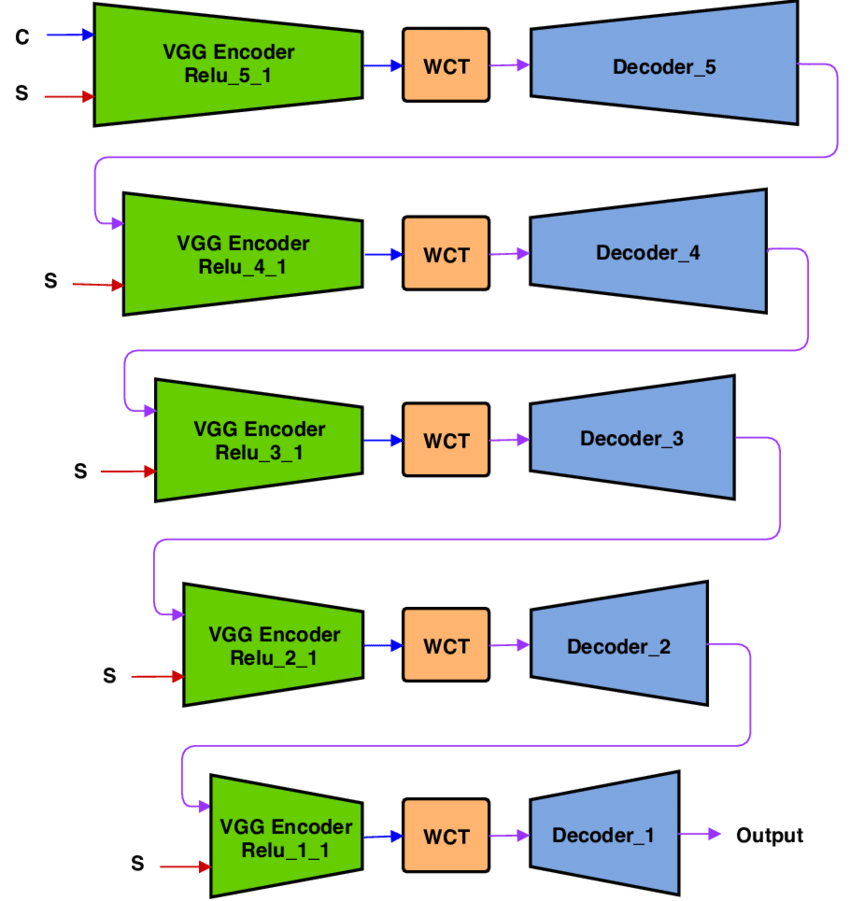
\includegraphics[width=\linewidth]{Universal-Style-Transfer-architecture-with-the-whole-multi-level-pipeline-Each-level-of.jpg}
		\caption{Encoder WCT Decoder Architecture}
	\end{subfigure}
	\begin{subfigure}[b]{0.4\linewidth}
		\includegraphics[width=\linewidth]{coffee.jpg}
		\caption{More coffee.}
	\end{subfigure}
	\caption{The same cup of coffee. Two times.}
	\label{fig:coffee}
\end{figure}
\newline
\newline\textbf{3.1  Stylization}\newline
\newline \textbf{WCT}. The WCT \cite{bib11} formulates stylization as an image reconstruction problem with feature projections. To utilize WCT, an auto-encoder for general image reconstruction is first trained. We used the VGG-19 model \cite{bib20} as the encoder $\varepsilon$(weights are kept fixed) and trains a decoder D for reconstructing the input image. The decoder is symmetrical to the encoder and uses up-sampling layers to enlarge the spatial resolutions of the feature maps,  (see figure 1.a). Once the auto-encoder is trained, a pair of projection functions are inserted at the network bottleneck to perform stylization through the whitening ($P_C$) and coloring ($P_S$) transforms. The key idea behind the WCT is to directly match feature correlations of the content image to those of the style image via the two projections. Specifically, given a pair of content image $I_C$ and style image $I_S$, the WCT first extracts their vectorised VGG features $C_f=\varepsilon(I_C)$ and $S_f=\varepsilon(I_S)$, and then transform the content feature $C_f$ via
\begin{equation}
CS_f = P_SP_CH_C
\end{equation}
Where $P_C=E_C\Lambda_C^{-\frac{1}{2}}$, and $P_S=E_S\Lambda_S^{\frac{1}{2}}$. Here $\Lambda_C$ and $\Lambda_S$ are the diagonal matrices with the eigenvalues of the covariance matrix $C_fC_f^T$ and $S_fS_f^T$ respectively. The matrices $E_C$ and $E_S$ are the corresponding orthonormal matrices of the eigenvalues, respectively. After the transformation, the correlations of
transformed features match those of the style features, i.e., $CS_fCS_f^T=S_fS_f^T$. Finally, the stylized image is obtained by directly feeding the transformed feature
map into the decoder: $Y = D(CS_f)$. For better stylization performance, Li et
al. \cite{bib11} use a multi-level stylization strategy, which performs the WCT on the
VGG features at different layers.
The WCT performs well for artistic image stylization. However it generates
structural artifacts (e.g., distortions on object boundaries)
	
	\section{Experiments}
	\label{experiments_lbl}
	%%%%%  Decoder %%%%%
\subsection{Reconstruction Quality Evaluation}

Our implementation of the Universal Style Transfer is adapted to use two different sets of encoder-decoder models: the models we trained according to section \ref{subsec:Models} (our), and the models offered to download by Li et al in their GitHub (reference). This means we can test \textbf{our implementation} of the UST algorithm with both sets of models. In this section we want to evaluate our models in comparison to the references in terms of image reconstruction, in order to asses the quality of our models training.

\subsubsection{Quantative Reconstruction Loss}
In order to quantify the reconstruction distortion induced by our trained models, in comparison to that of the reference models, we encode and then decode 1k content images from the COCO dataset using all 5 encoder-decoder pairs, and measure the pixel MSE and feature MSE. The pixel MSE measures the mean square error between the reconstructed image, $\hat{x}$, and the original one, $x$, i.e. $MSE(x - \hat{x})$. The feature MSE measures the error between the deep features of the reconstructed image and the original one. It is measured by again encoding $x$ and $\hat{x}$ and calculating $MSE(E(x)-E(\hat{x}))$. Table ~\ref{Tab:loss} displays the pixel loss (feature loss) per model, which are defined to be the average pixel MSE (feature MSE) over the 1k images.

% ecoder-decoder table %

\begin{center}
	\captionof{table}{Pixel and Feature Loss Per Model\label{Tab:loss}}
	\centering
	\begin{tabular}{ |>{\centering}p{2.5cm}||>{\centering}p{2.5cm}|>{\centering}p{2.5cm}|>{\centering}p{2.5cm}|>{\centering}p{2.5cm}| }
		\hline
		\multicolumn{5}{|c|}{\hspace{1.4cm} Pixel loss[$1\mathrm{e}{-4}$] \hspace{3cm}$\mid$ \hspace{1cm} Feature loss[$1\mathrm{e}{-2}$]} \\
		\hline
		architecture &Reference &Our &Reference &Our \tabularnewline
		\hline
		1 &$8.246$  &$802$   &$2.161$ &$0.7$\tabularnewline
		\hline
		2 &$2.374$  &$810$   &$1.257$ &$15.30$\tabularnewline
		\hline
		3 &$7.994$  &$884$   &$16.38$ &$86.60$\tabularnewline
		\hline
		4 &$0.281$  &$830$   &$25.09$ &$223.6$\tabularnewline
		\hline
		5 &$..$  &$..$   &$..$ &..\tabularnewline
		\hline
	\end{tabular}\\
\end{center}

\subsubsection{Qualitative Reconstruction Loss}
To demonstrate the image reconstruction performance of our trained models, we choose 5 different images and feed them as input to our encoder-decoder architectures, as well as to the reference architectures. The results, as presented in figure ~\ref{fig:reconstruction}, visualize the image reconstruction quality of our models in comparison to that of the references.\newline
In figure ~\ref{fig:reconstruction} (a) we present Our reconstruction which means the use of trained decoders as in VGG-19 \cite{bib20} and encoder, based on torchvision package.
As can be visually seen, our reconstruction images are less good than Li et al. \cite{bib11} results. Our results suffer from artifacts such as blurring and over smoothing, especially in small details such as faces. This artifacts are outcome of our trained decoder.

\begin{figure}[H]
	% first line
	\centering
	\begin{subfigure}[b]{0.13\linewidth}
		
\includegraphics[width=\linewidth]{bridge_sq.jpg} % original num.1	
	\end{subfigure}
	\begin{subfigure}[b]{0.13\linewidth}
		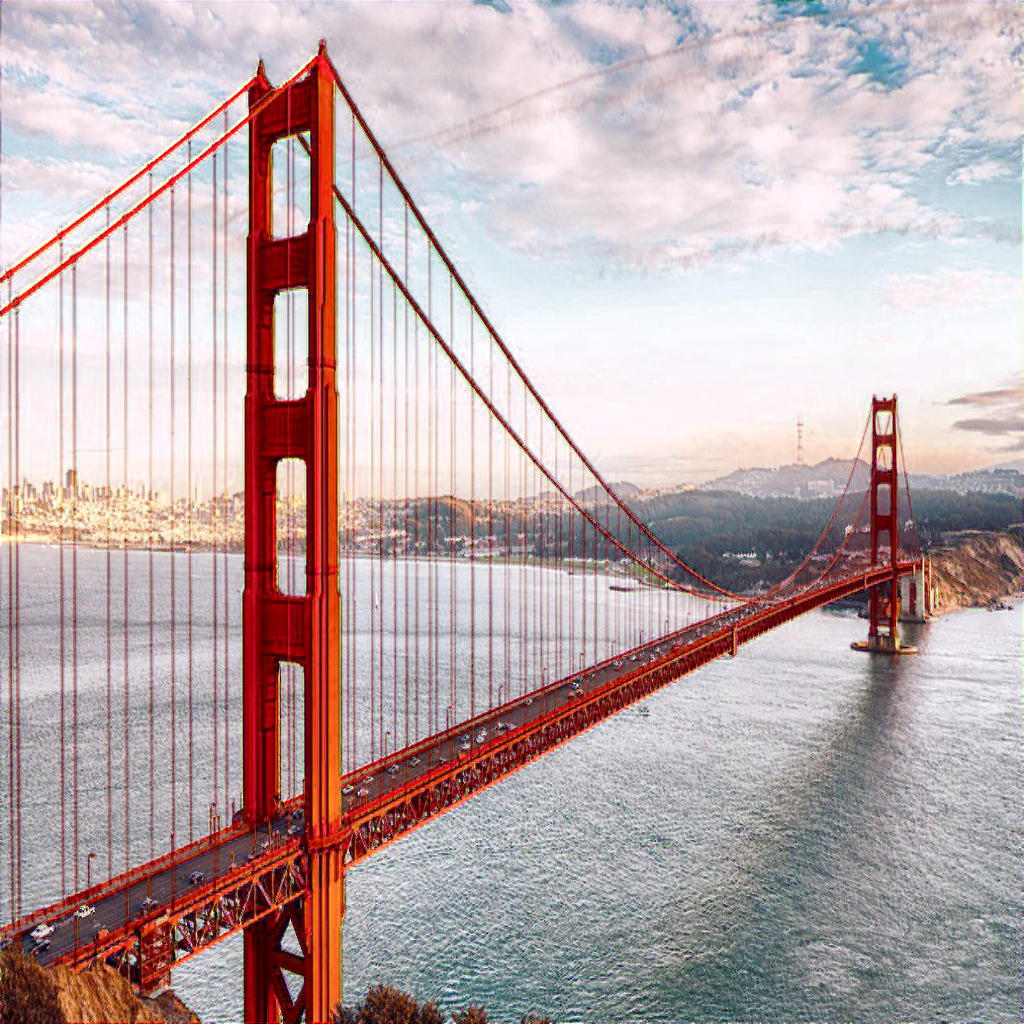
\includegraphics[width=\linewidth]{reconst_exper/dec_bridge_my_1_test.png} % our reconstruction arc1 num.1	
	\end{subfigure}
	\begin{subfigure}[b]{0.13\linewidth}
		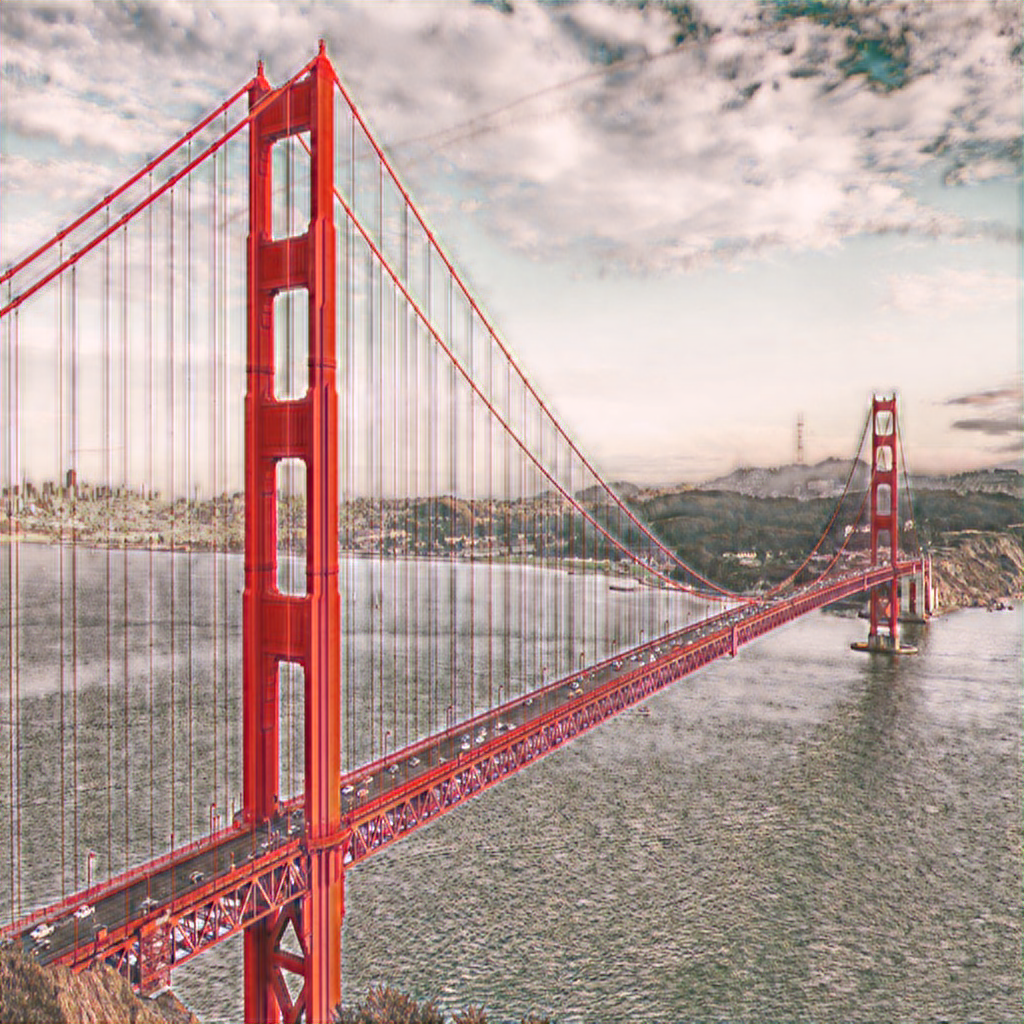
\includegraphics[width=\linewidth]{reconst_exper/dec_bridge_my_2_test.png} % our reconstruction arc2 num.1	
	\end{subfigure}
	\begin{subfigure}[b]{0.13\linewidth}
		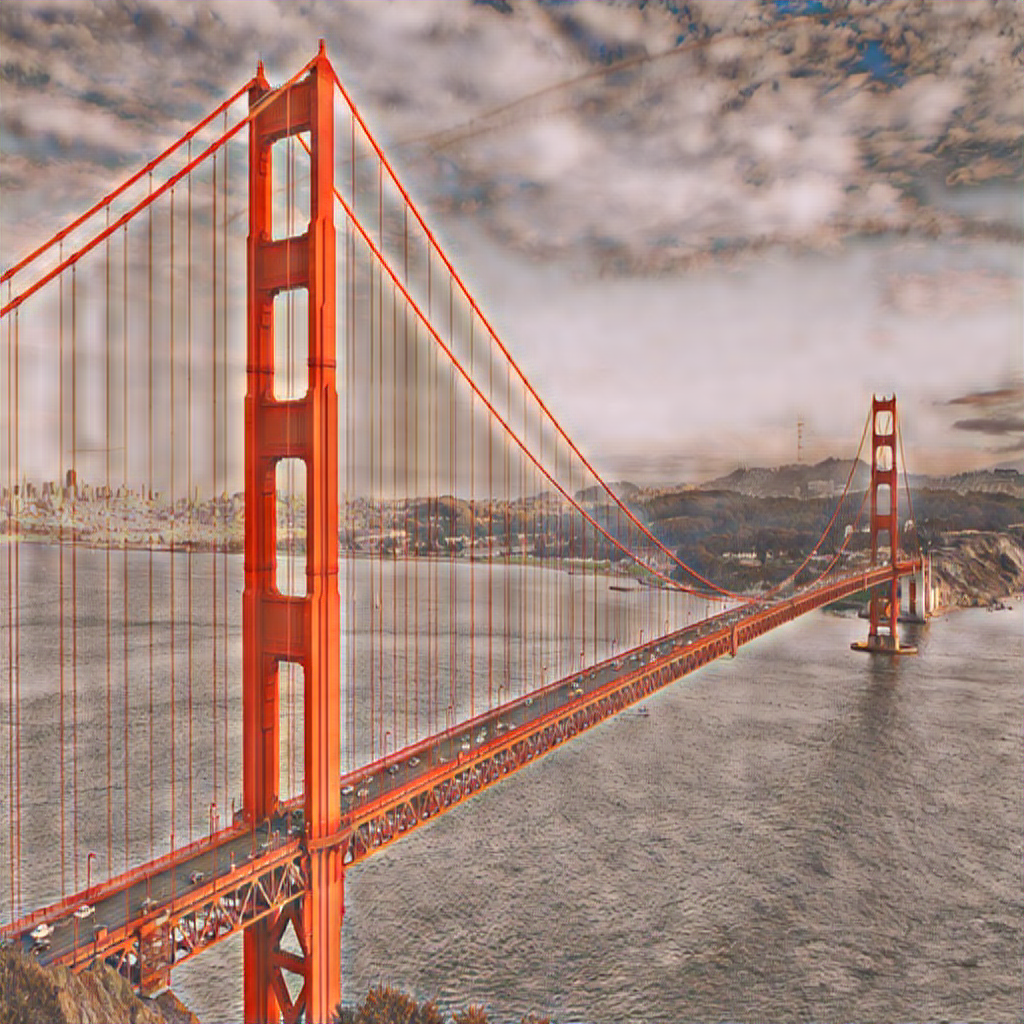
\includegraphics[width=\linewidth]{reconst_exper/dec_bridge_my_3_test.png} % our reconstruction arc3 num.1	
	\end{subfigure}
	\begin{subfigure}[b]{0.13\linewidth}
		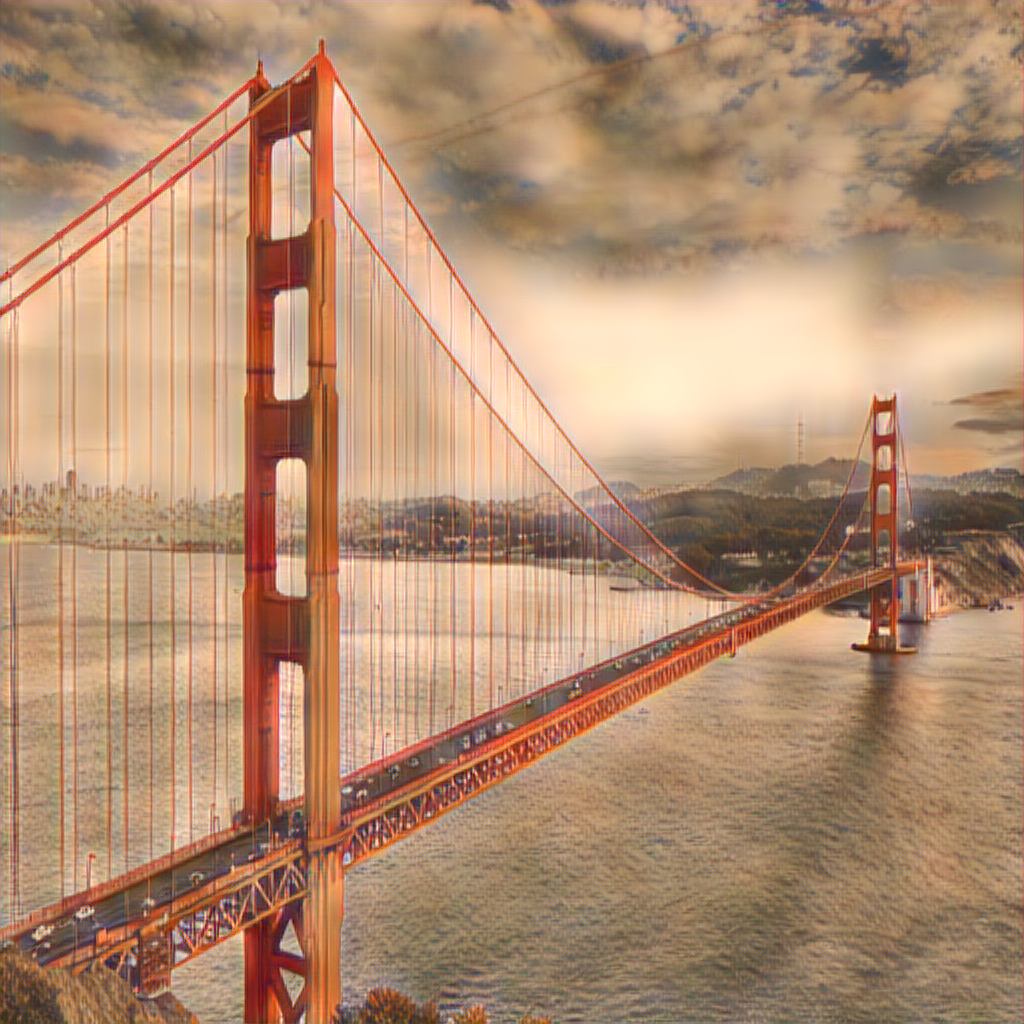
\includegraphics[width=\linewidth]{reconst_exper/dec_bridge_my_4_test.png} % our reconstruction arc4 num.1	
	\end{subfigure}
	\begin{subfigure}[b]{0.13\linewidth}
		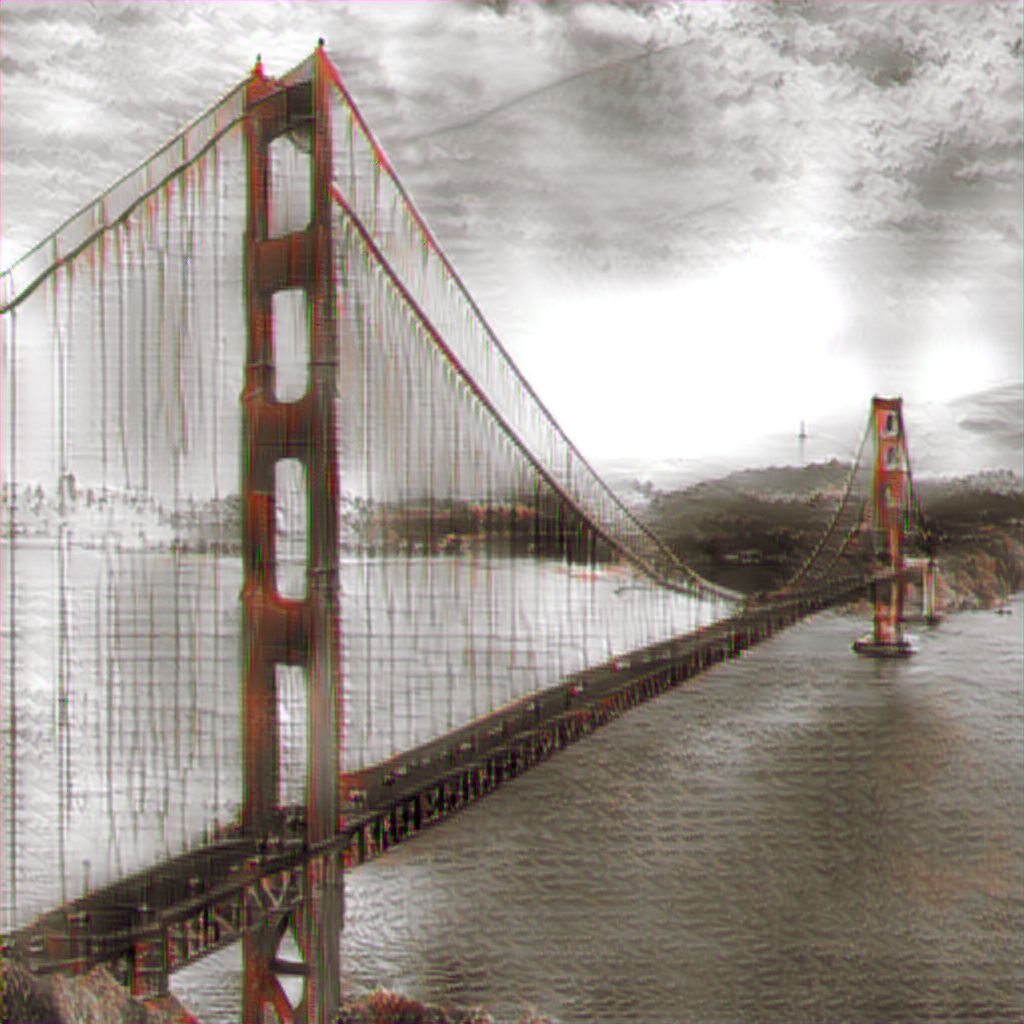
\includegraphics[width=\linewidth]{reconst_exper/dec_bridge_my_5_test.png} % our reconstruction arc5 num.1	
	\end{subfigure}
	\begin{subfigure}[b]{0.13\linewidth}
		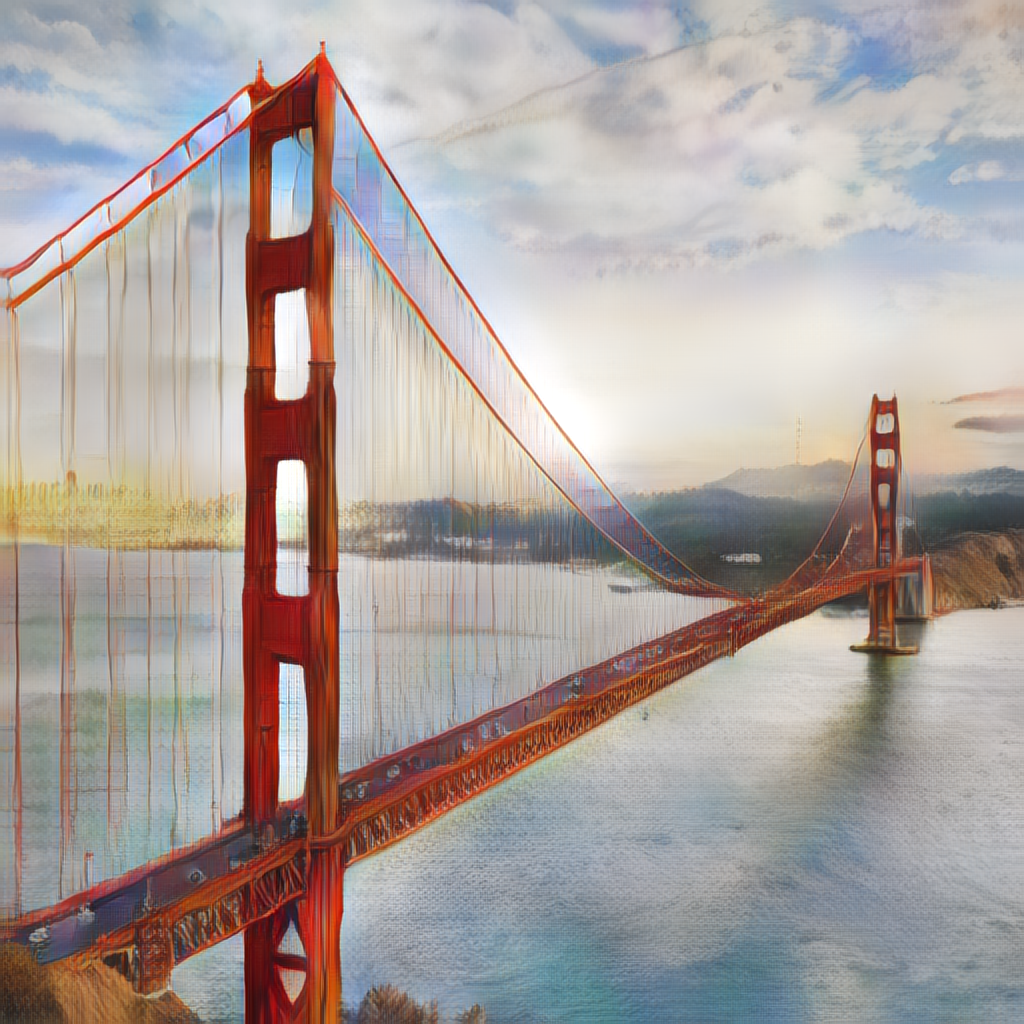
\includegraphics[width=\linewidth]{reconst_exper/dec_bridge_ref_5_test.png} % their reconstruction arc5 num.1	
	\end{subfigure}
	% second line
	\centering
	\begin{subfigure}[b]{0.13\linewidth}
		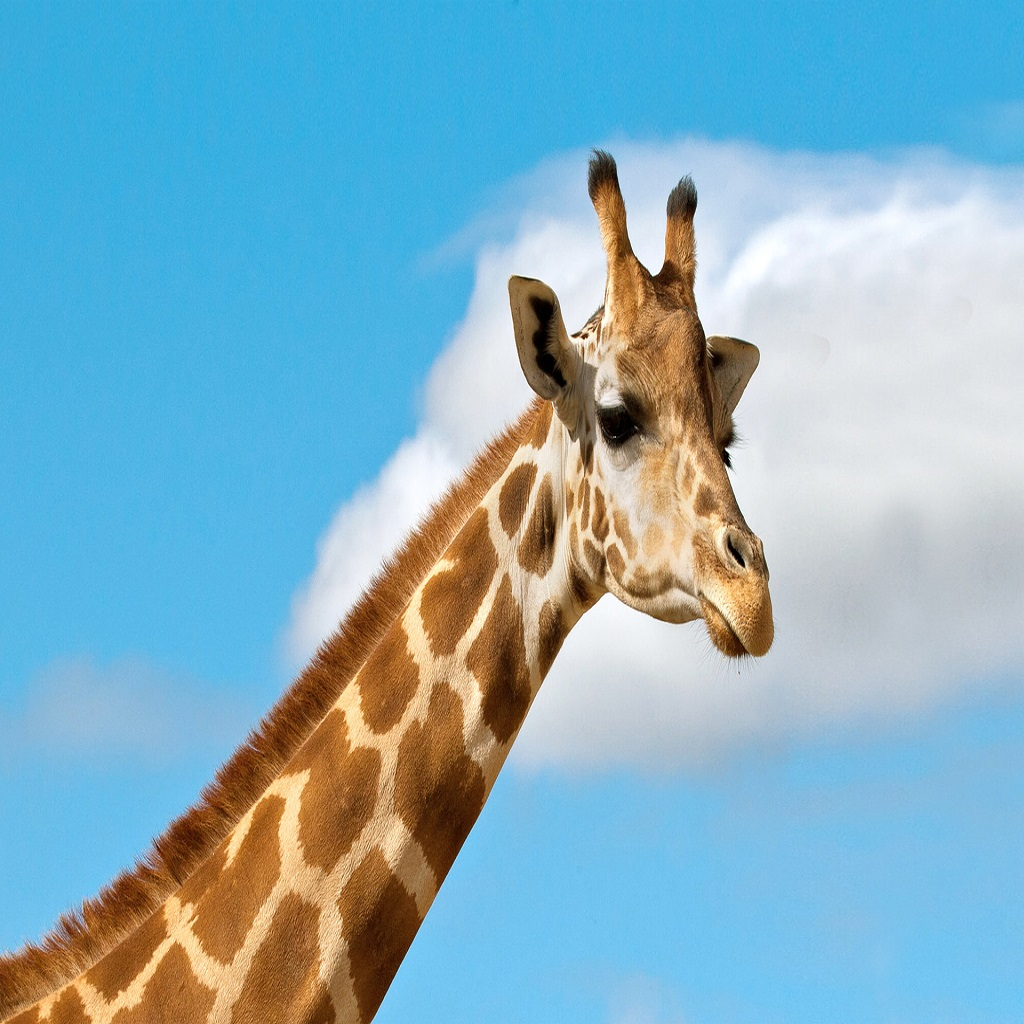
\includegraphics[width=\linewidth]{giraffe_sq.jpg} % original num.1	
	\end{subfigure}
	\begin{subfigure}[b]{0.13\linewidth}
		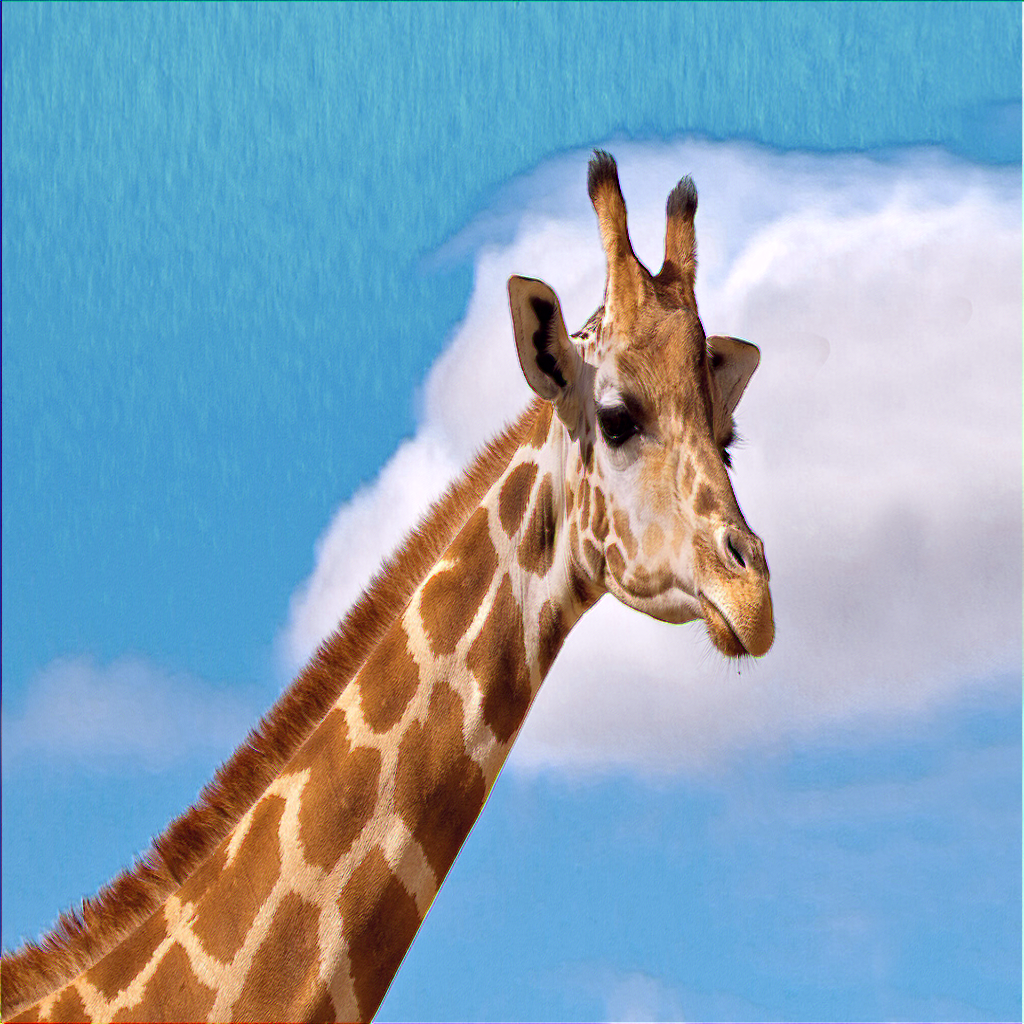
\includegraphics[width=\linewidth]{reconst_exper/dec_giraffe_my_1_test.png} % our reconstruction arc1 num.1	
	\end{subfigure}
	\begin{subfigure}[b]{0.13\linewidth}
		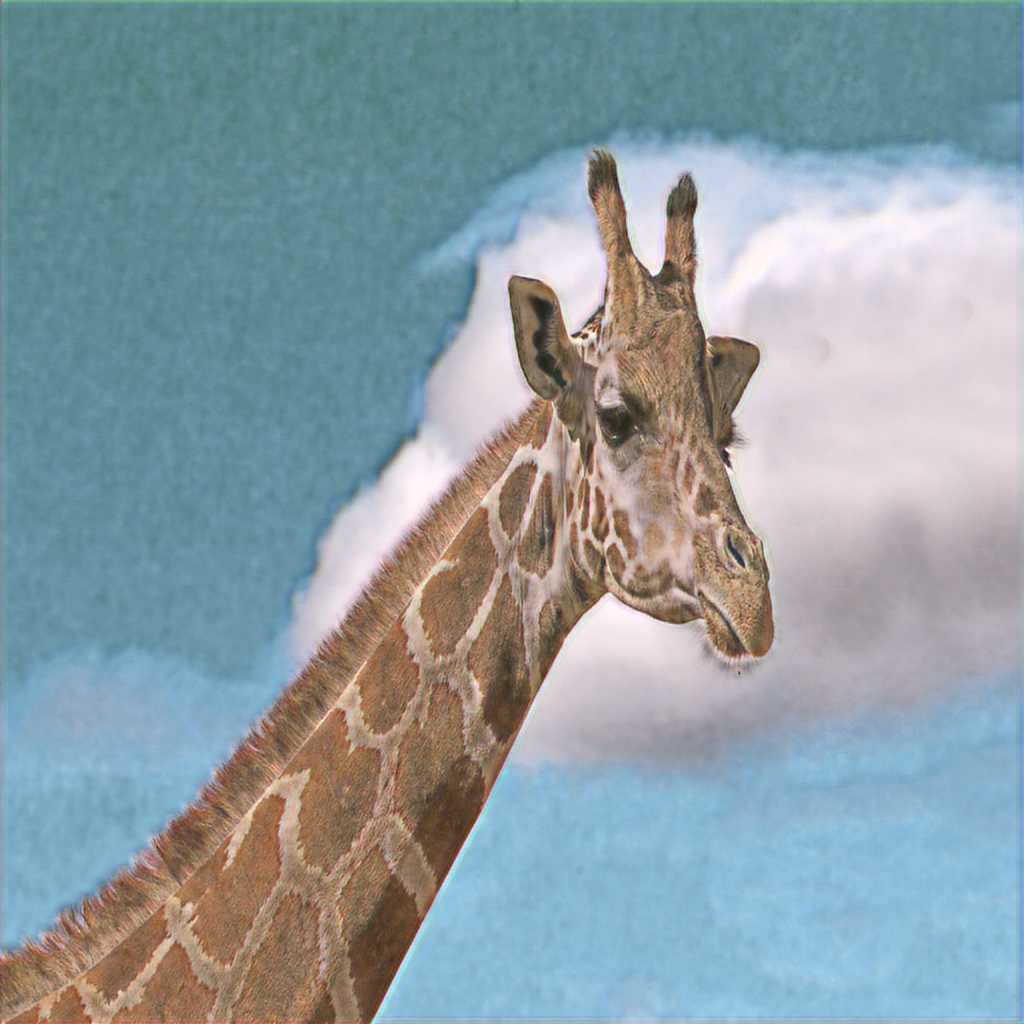
\includegraphics[width=\linewidth]{reconst_exper/dec_giraffe_my_2_test.png} % our reconstruction arc2 num.1	
	\end{subfigure}
	\begin{subfigure}[b]{0.13\linewidth}
		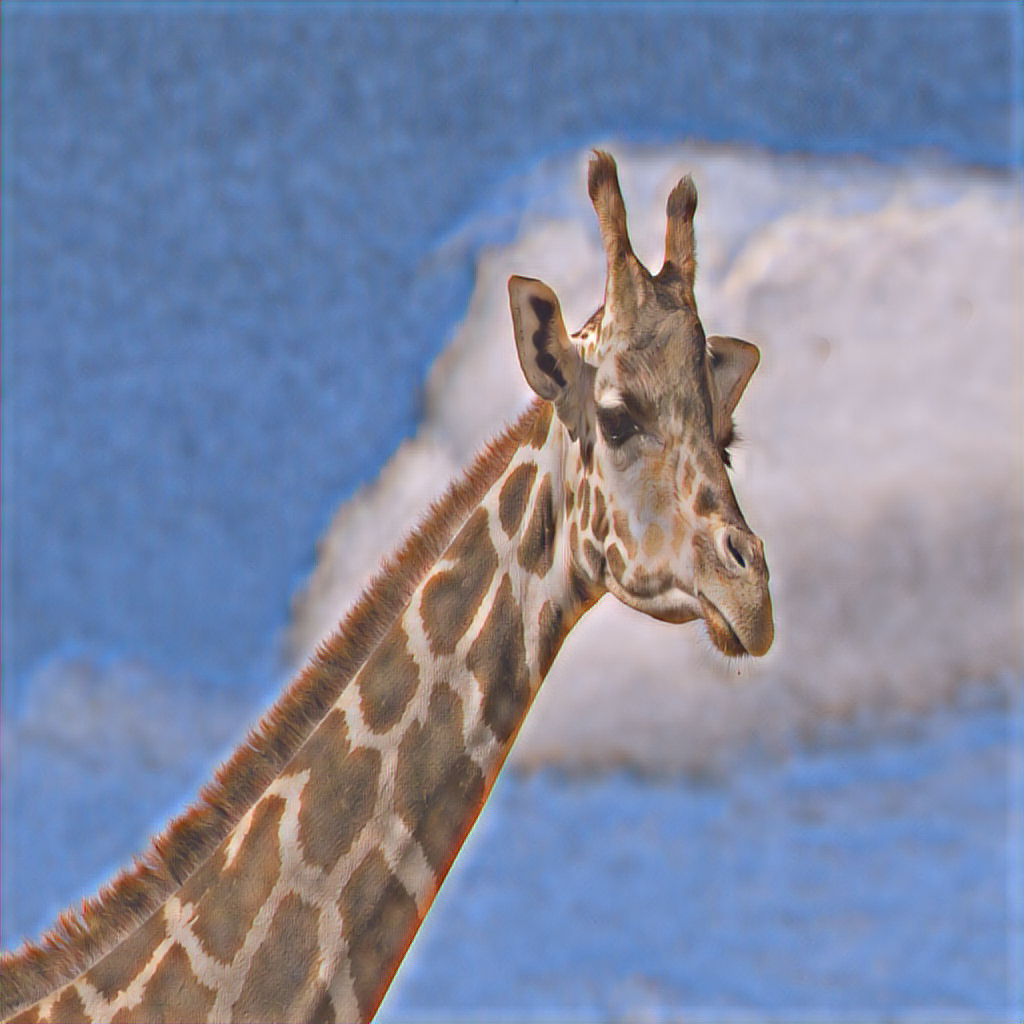
\includegraphics[width=\linewidth]{reconst_exper/dec_giraffe_my_3_test.png} % our reconstruction arc3 num.1	
	\end{subfigure}
	\begin{subfigure}[b]{0.13\linewidth}
		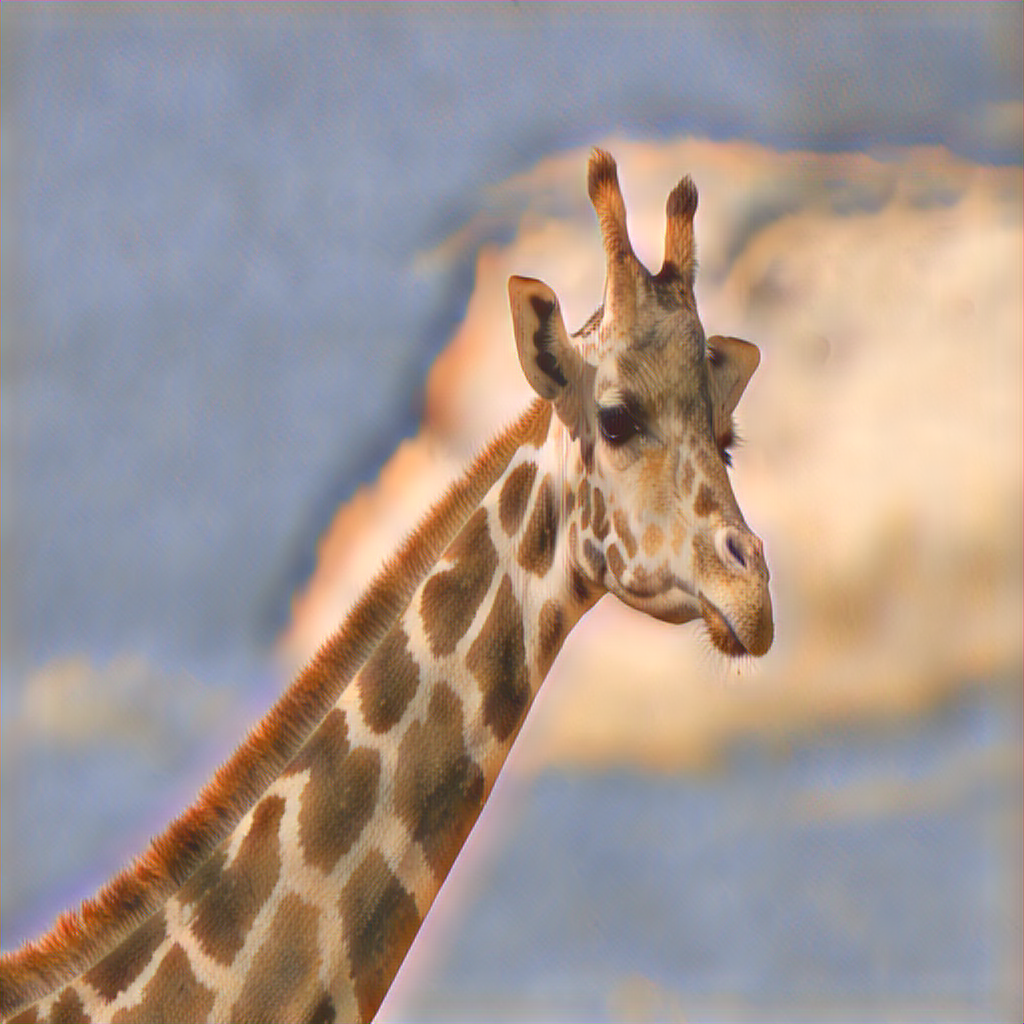
\includegraphics[width=\linewidth]{reconst_exper/dec_giraffe_my_4_test.png} % our reconstruction arc4 num.1	
	\end{subfigure}
	\begin{subfigure}[b]{0.13\linewidth}
		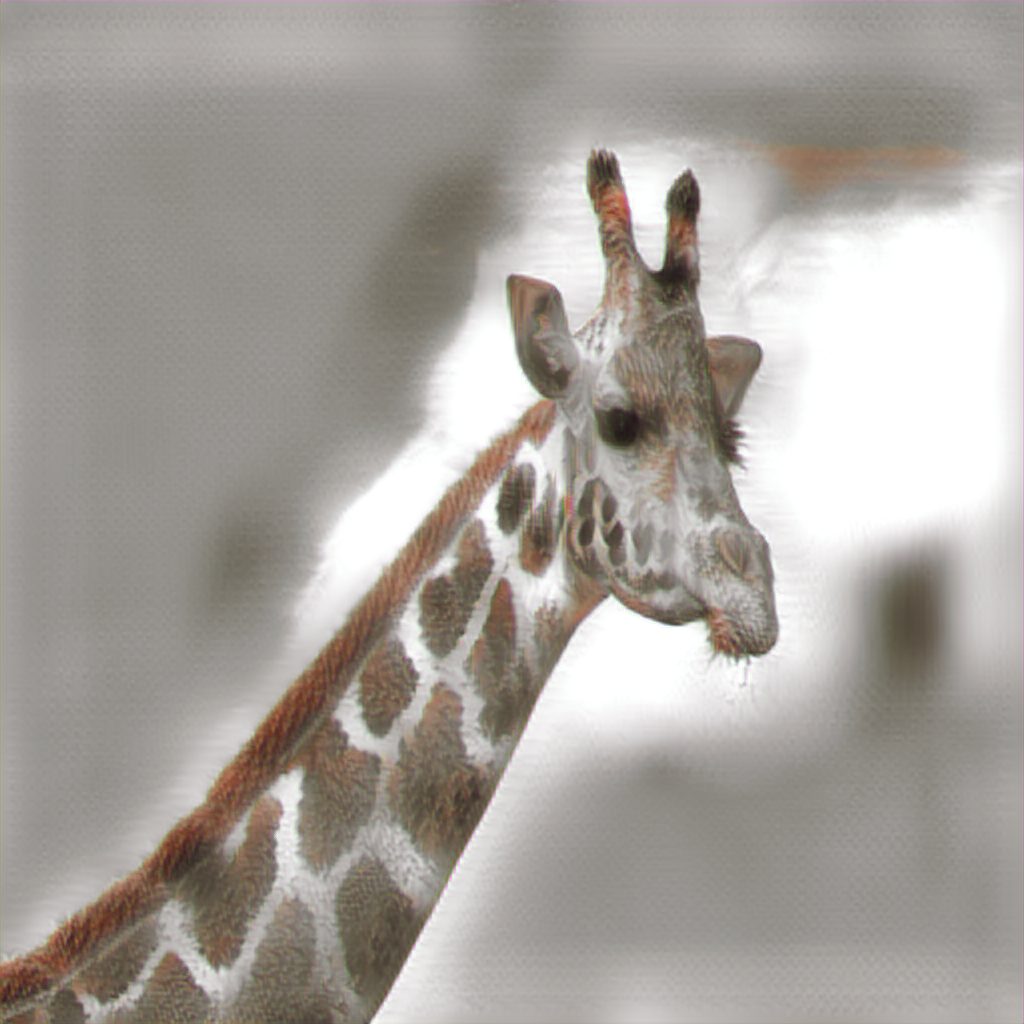
\includegraphics[width=\linewidth]{reconst_exper/dec_giraffe_my_5_test.png} % our reconstruction arc5 num.1	
	\end{subfigure}
	\begin{subfigure}[b]{0.13\linewidth}
		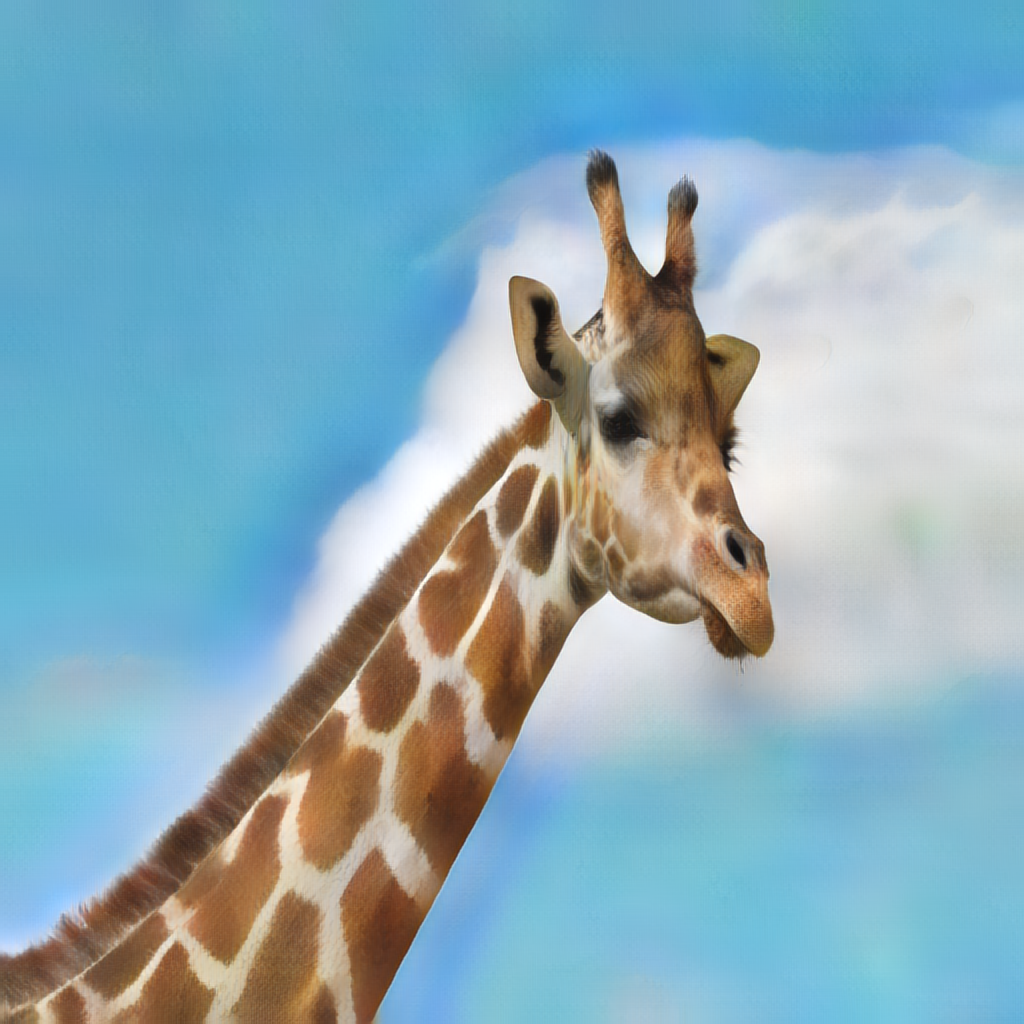
\includegraphics[width=\linewidth]{reconst_exper/dec_giraffe_ref_5_test.png} % their reconstruction arc5 num.1	
	\end{subfigure}
	% third line
	\centering
	\begin{subfigure}[b]{0.13\linewidth}
		
\includegraphics[width=\linewidth]{in1_sq.jpg} % original num.1	
	\end{subfigure}
	\begin{subfigure}[b]{0.13\linewidth}
		
\includegraphics[width=\linewidth]{reconst_exper/dec_in1_my_1_test.png} % our reconstruction arc1 num.1	
	\end{subfigure}
	\begin{subfigure}[b]{0.13\linewidth}
		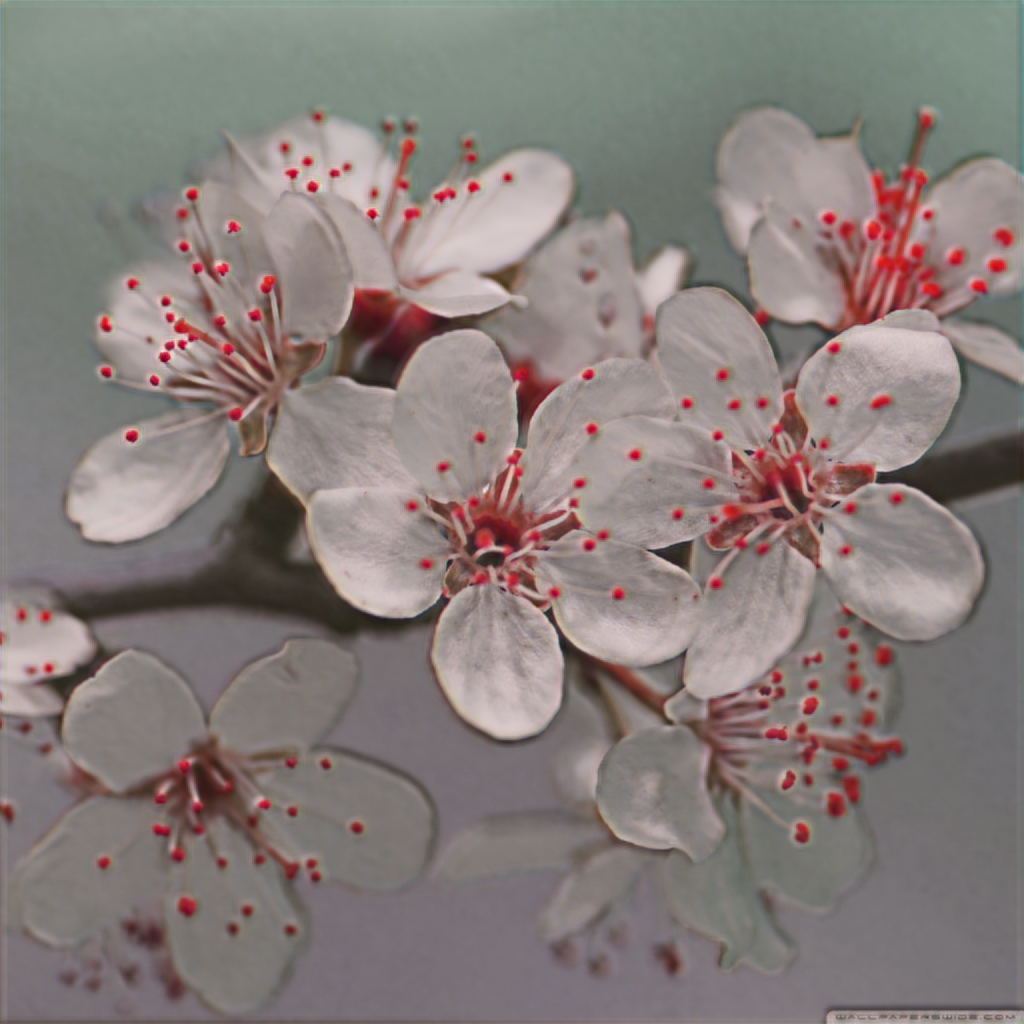
\includegraphics[width=\linewidth]{reconst_exper/dec_in1_my_2_test.png} % our reconstruction arc2 num.1	
	\end{subfigure}
	\begin{subfigure}[b]{0.13\linewidth}
		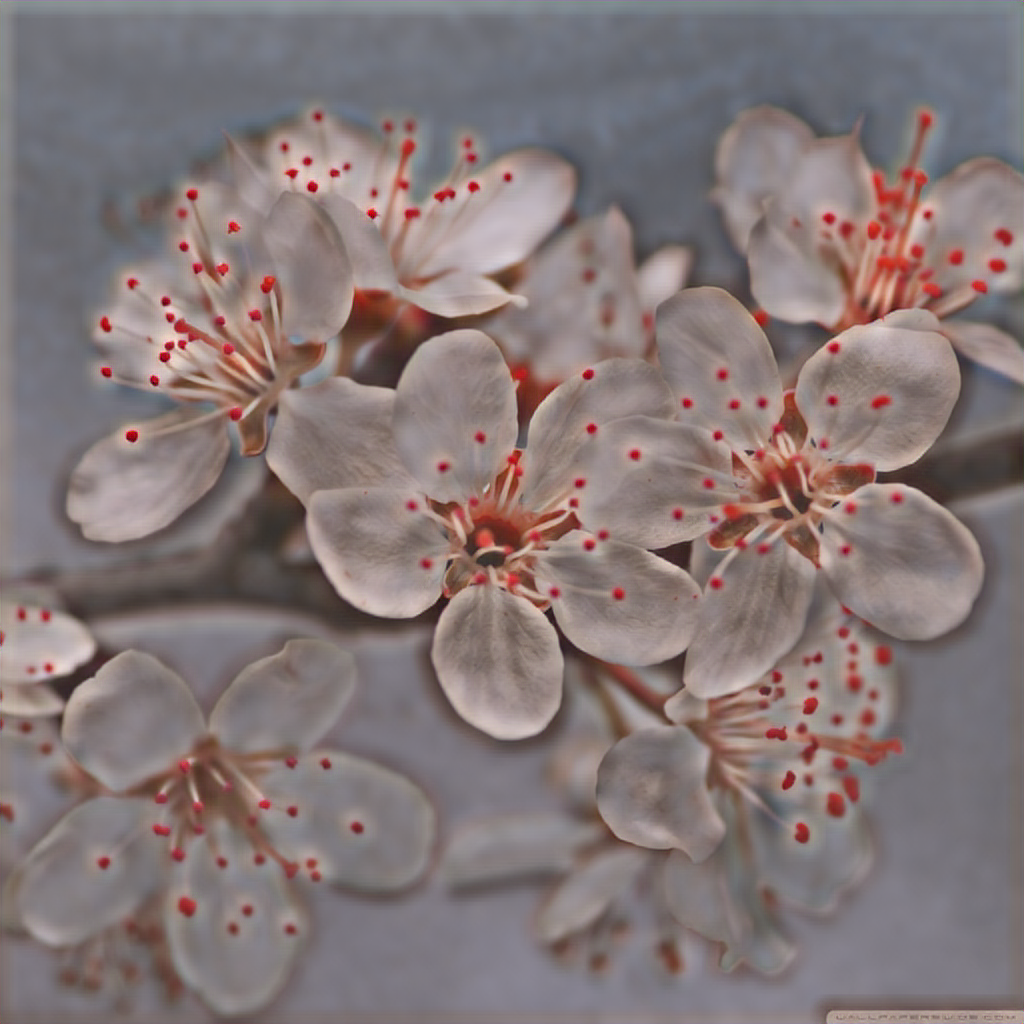
\includegraphics[width=\linewidth]{reconst_exper/dec_in1_my_3_test.png} % our reconstruction arc3 num.1	
	\end{subfigure}
	\begin{subfigure}[b]{0.13\linewidth}
		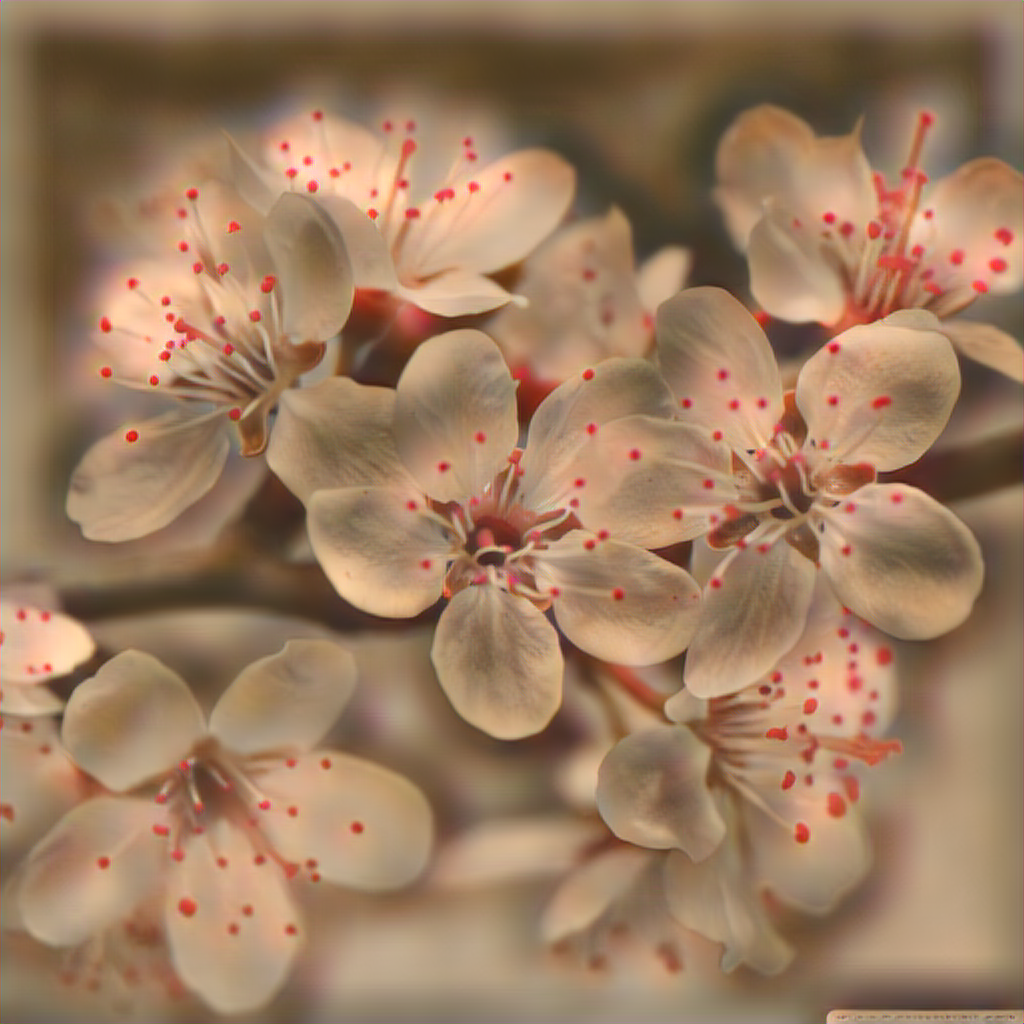
\includegraphics[width=\linewidth]{reconst_exper/dec_in1_my_4_test.png} % our reconstruction arc4 num.1	
	\end{subfigure}
	\begin{subfigure}[b]{0.13\linewidth}
		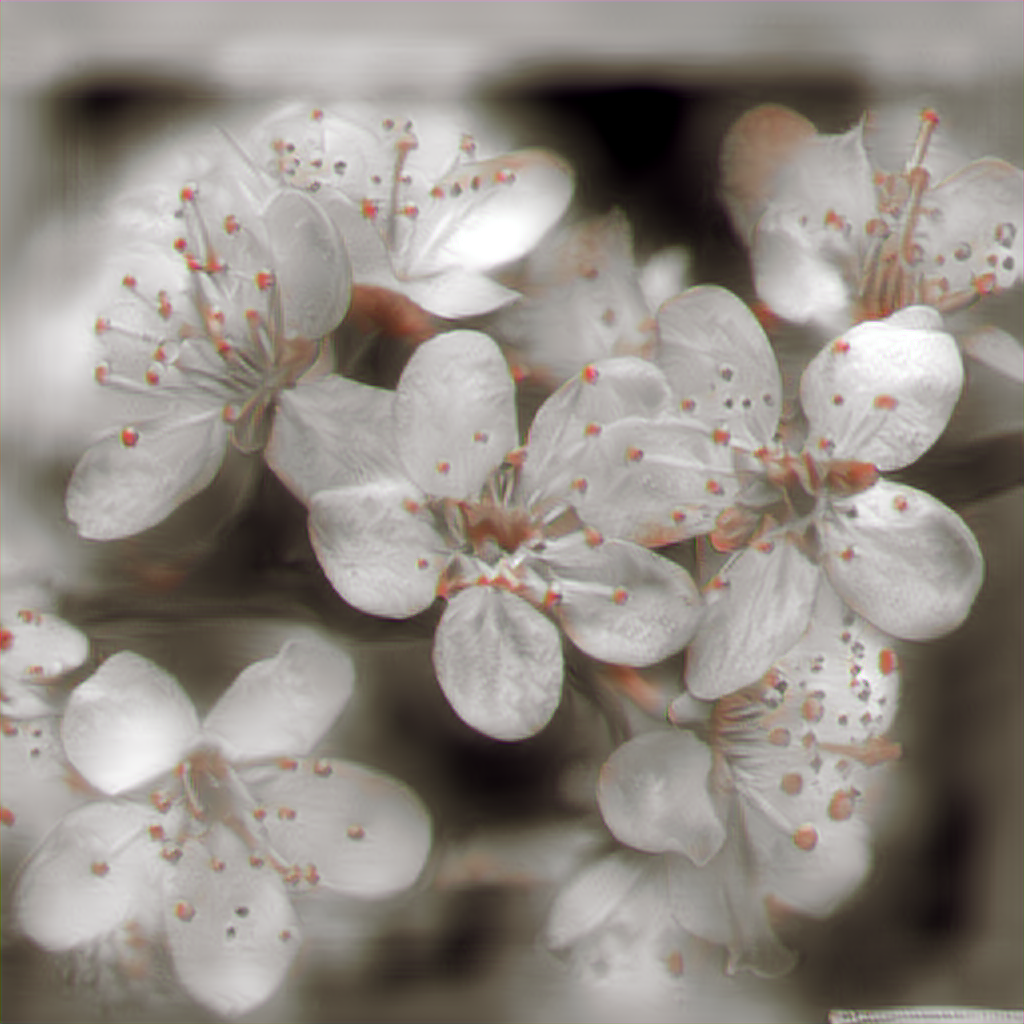
\includegraphics[width=\linewidth]{reconst_exper/dec_in1_my_5_test.png} % our reconstruction arc5 num.1	
	\end{subfigure}
	\begin{subfigure}[b]{0.13\linewidth}
		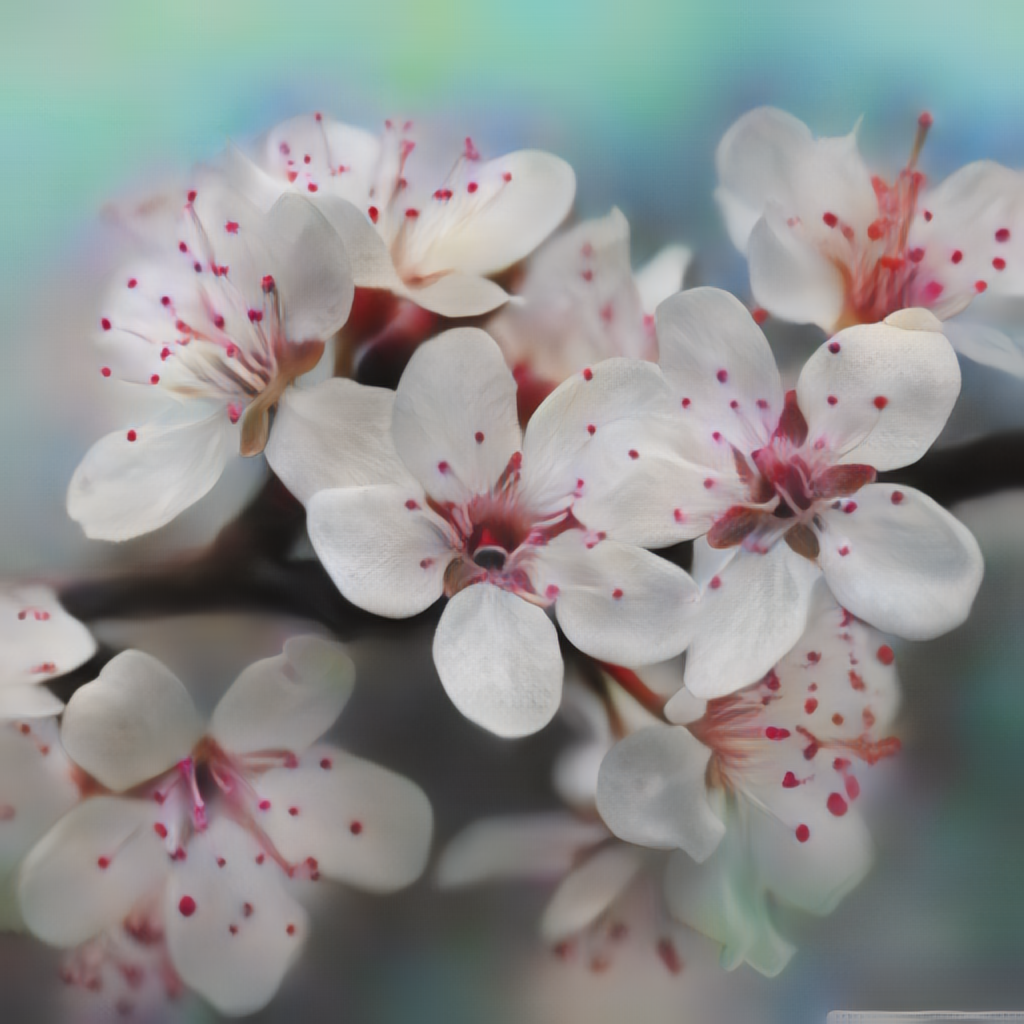
\includegraphics[width=\linewidth]{reconst_exper/dec_in1_ref_5_test.png} % their reconstruction arc5 num.1	
	\end{subfigure}
	%fourth line
	\centering
	\begin{subfigure}[b]{0.13\linewidth}
		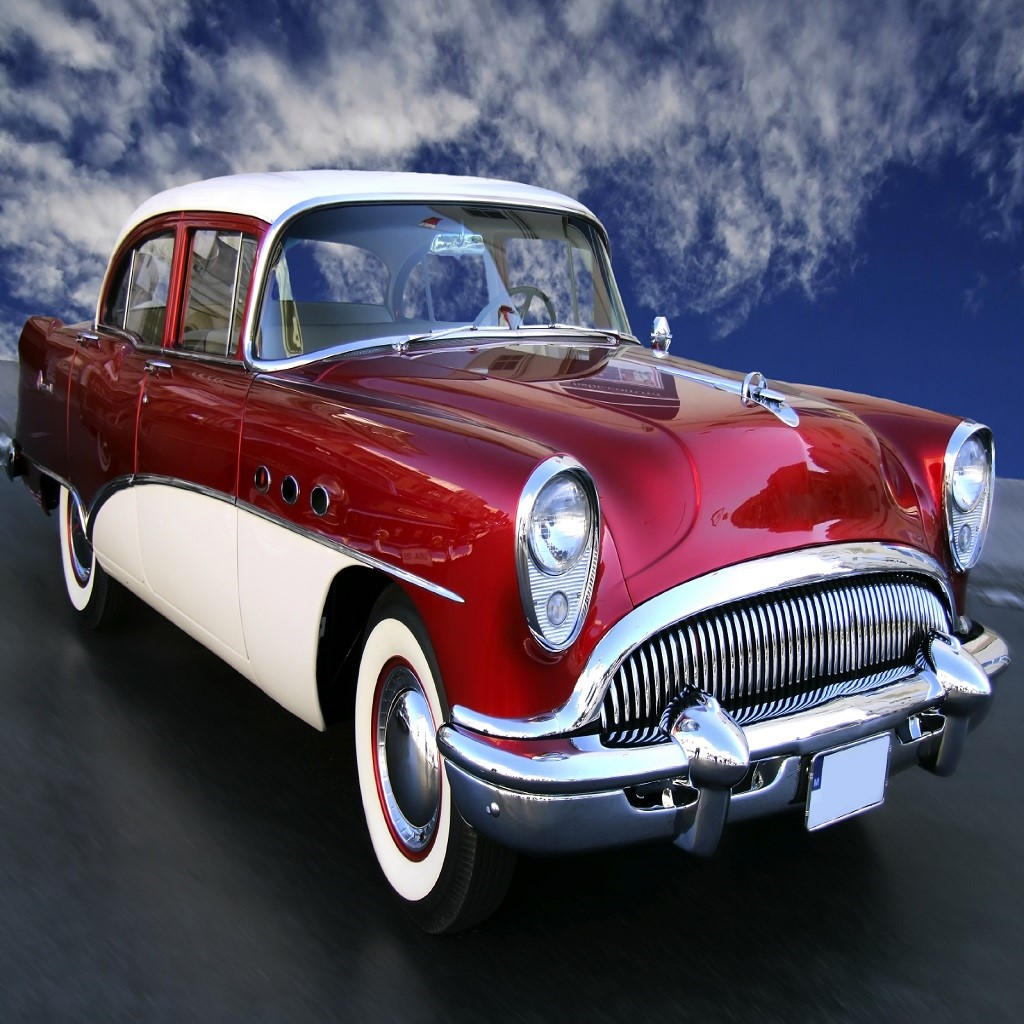
\includegraphics[width=\linewidth]{car_sq.jpg} % original num.1	
	\end{subfigure}
	\begin{subfigure}[b]{0.13\linewidth}
		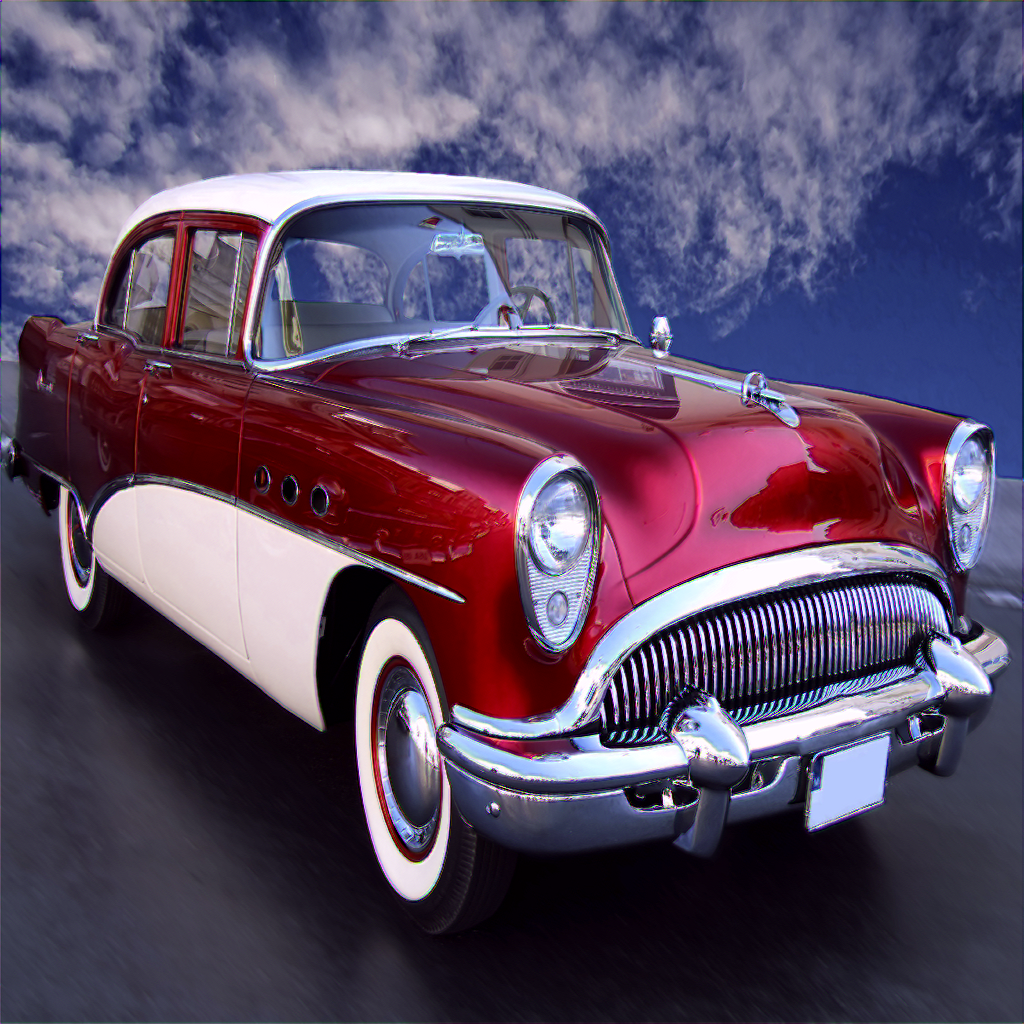
\includegraphics[width=\linewidth]{reconst_exper/dec_in2_my_1_test.png} % our reconstruction arc1 num.1	
	\end{subfigure}
	\begin{subfigure}[b]{0.13\linewidth}
		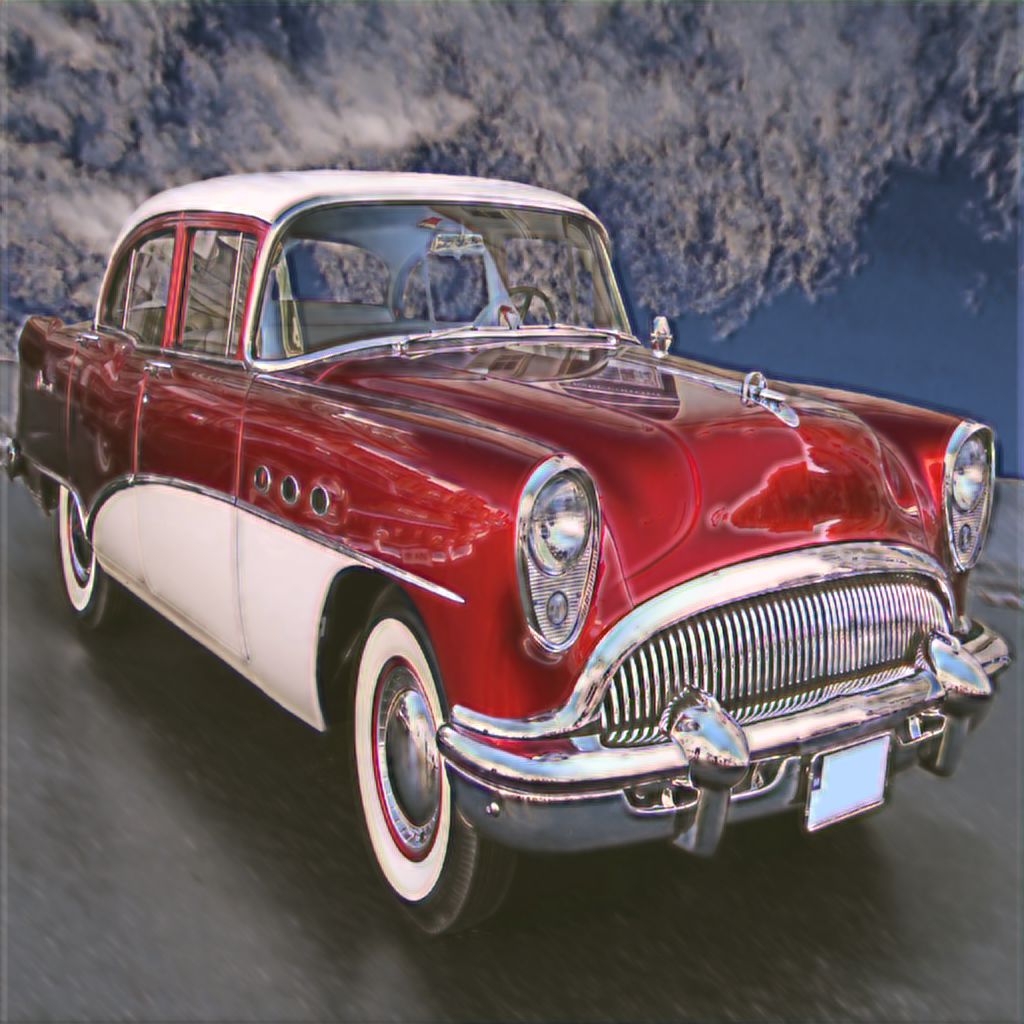
\includegraphics[width=\linewidth]{reconst_exper/dec_in2_my_2_test.png} % our reconstruction arc2 num.1	
	\end{subfigure}
	\begin{subfigure}[b]{0.13\linewidth}
		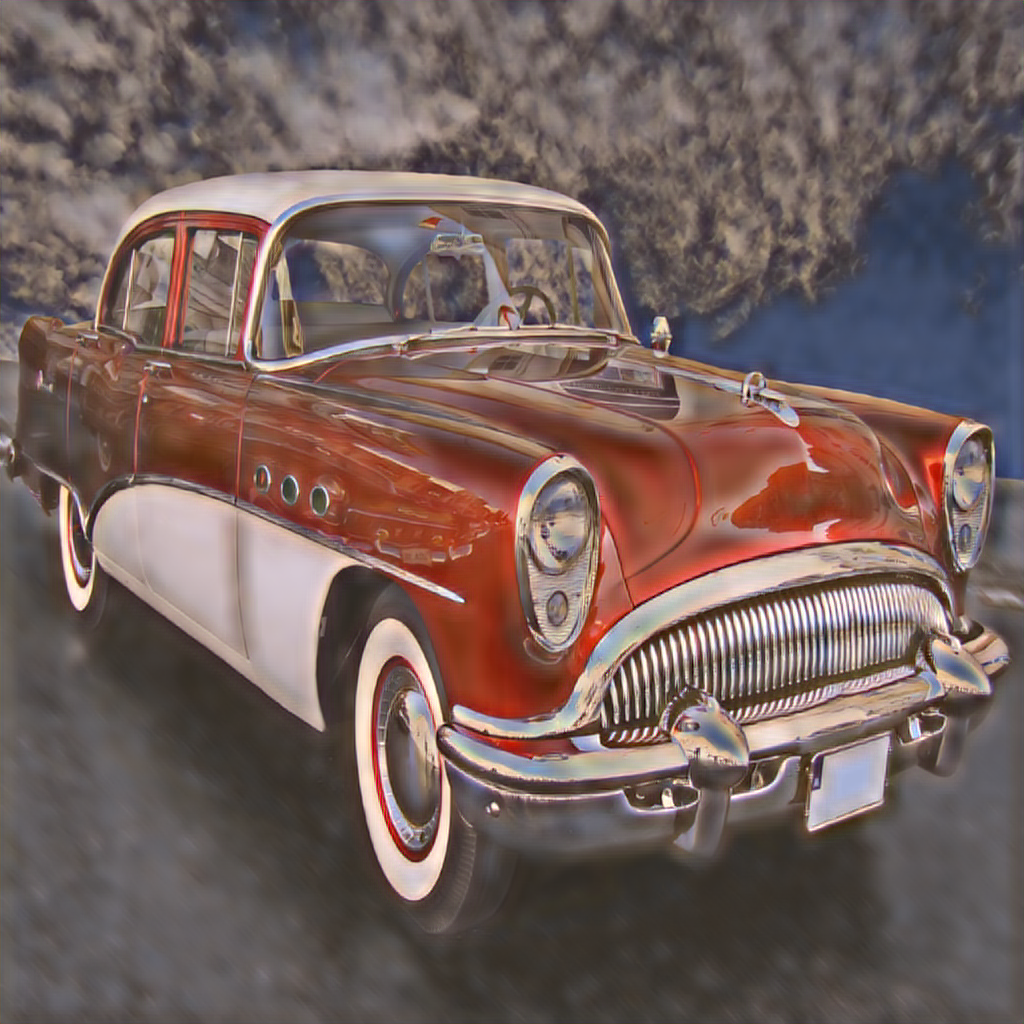
\includegraphics[width=\linewidth]{reconst_exper/dec_in2_my_3_test.png} % our reconstruction arc3 num.1	
	\end{subfigure}
	\begin{subfigure}[b]{0.13\linewidth}
		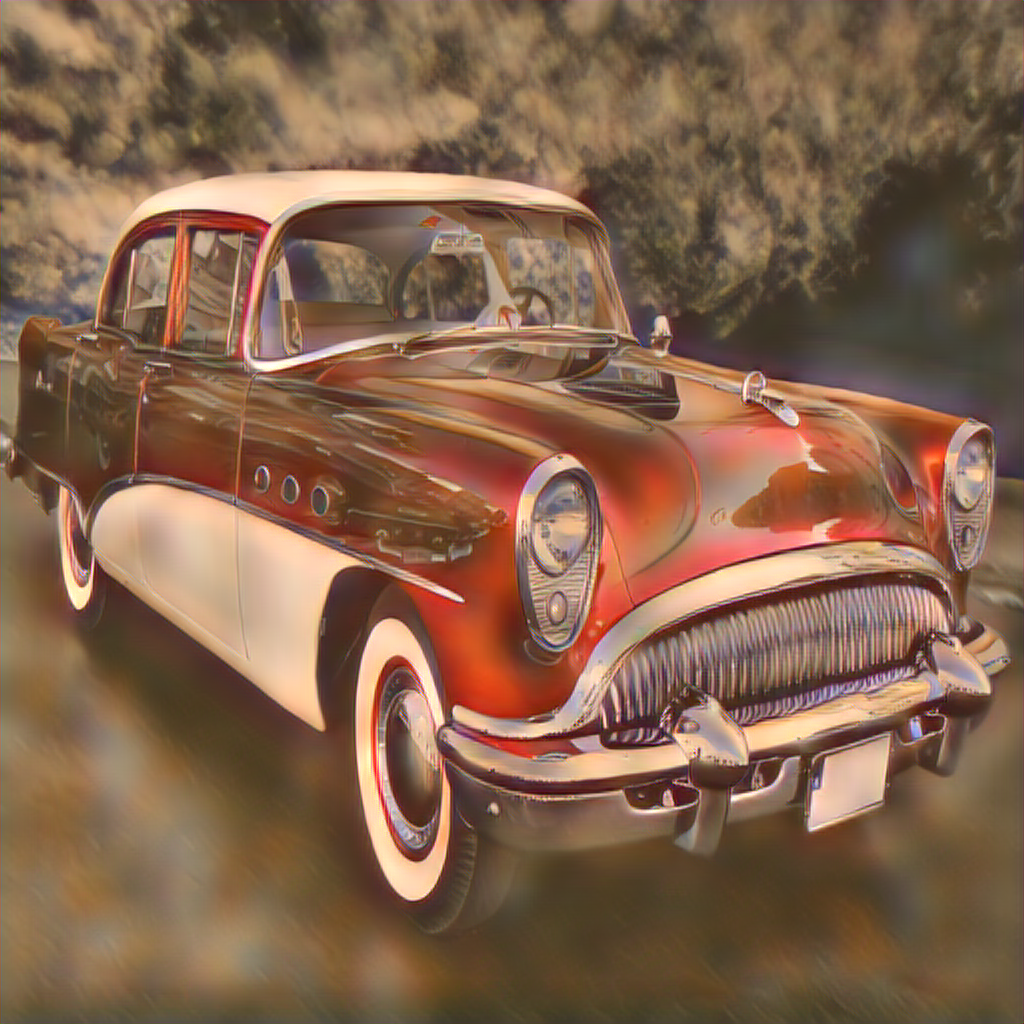
\includegraphics[width=\linewidth]{reconst_exper/dec_in2_my_4_test.png} % our reconstruction arc4 num.1	
	\end{subfigure}
	\begin{subfigure}[b]{0.13\linewidth}
		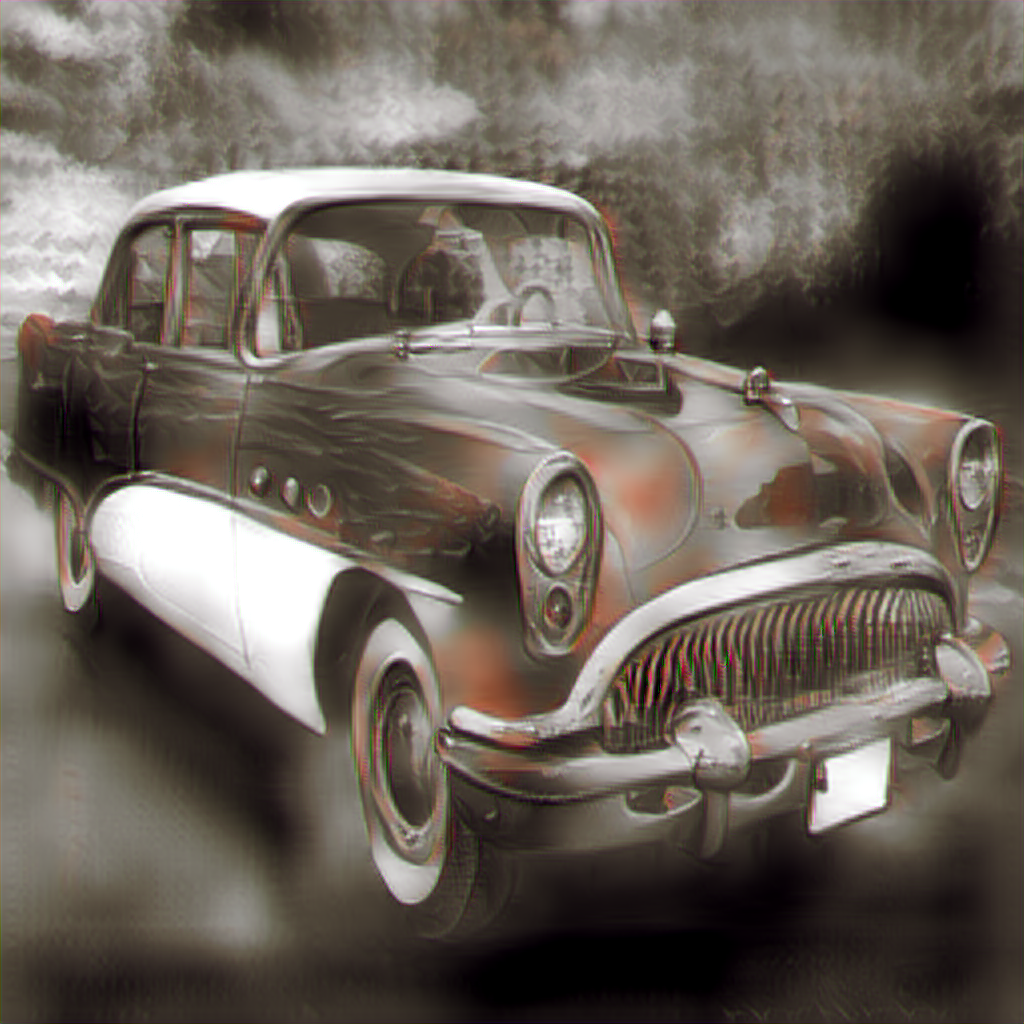
\includegraphics[width=\linewidth]{reconst_exper/dec_in2_my_5_test.png} % our reconstruction arc5 num.1	
	\end{subfigure}
	\begin{subfigure}[b]{0.13\linewidth}
		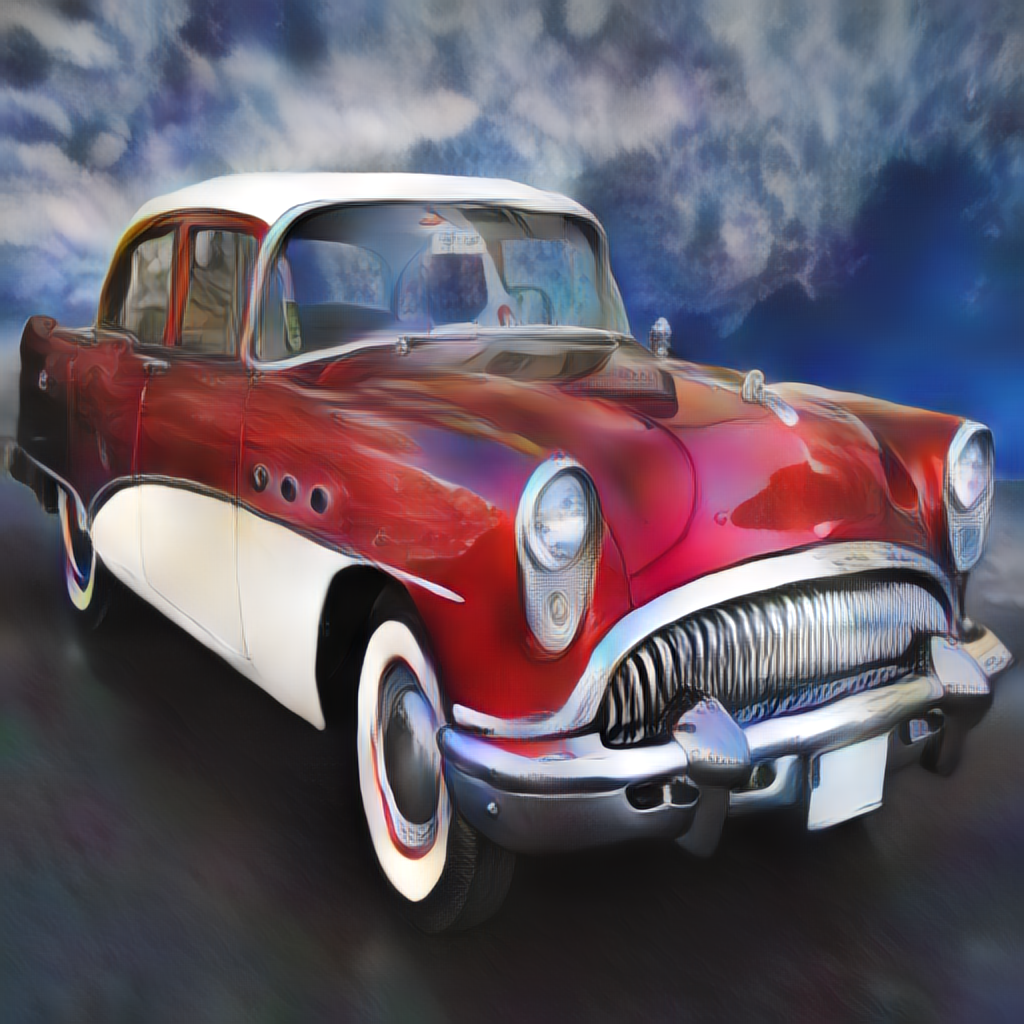
\includegraphics[width=\linewidth]{reconst_exper/dec_in2_ref_5_test.png} % their reconstruction arc5 num.1	
	\end{subfigure}
	% fifth line
	\centering
	\begin{subfigure}[b]{0.13\linewidth}
		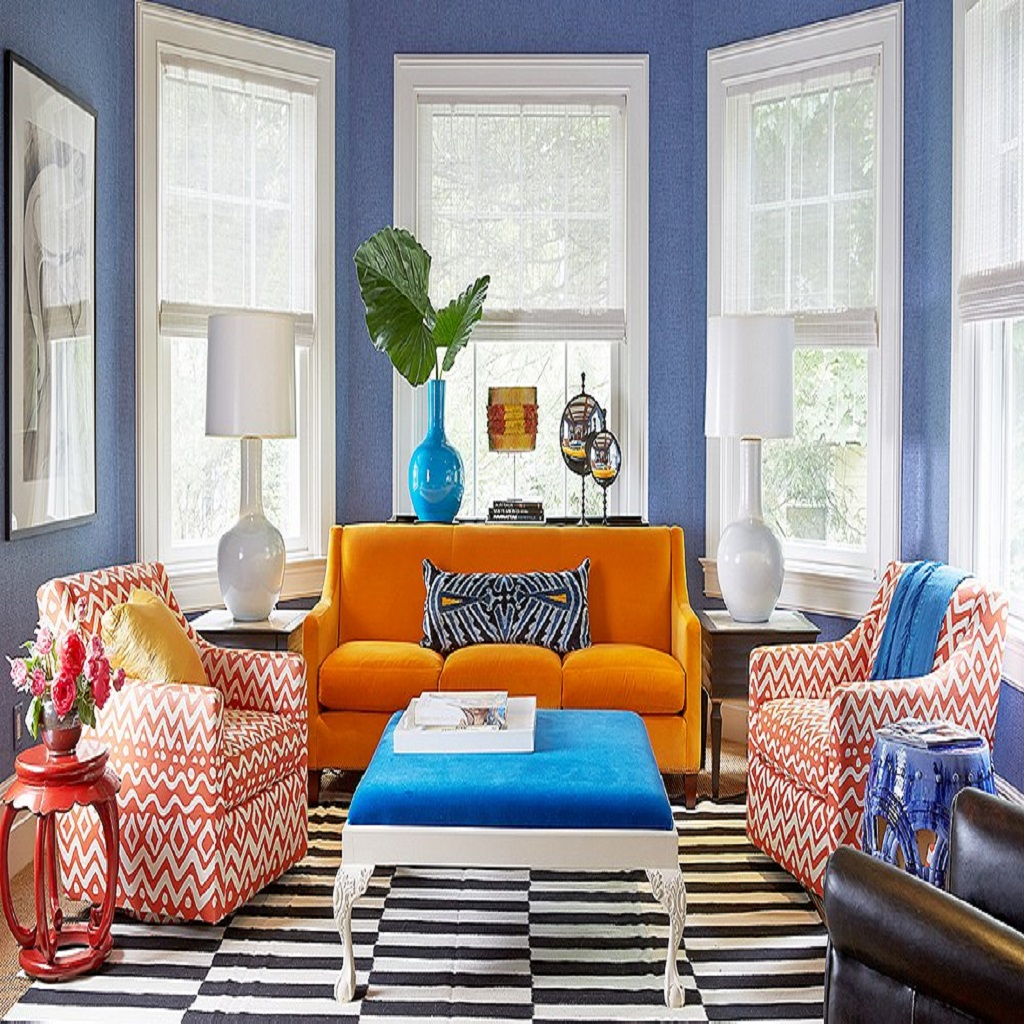
\includegraphics[width=\linewidth]{room_sq.jpg} % original num.5
		\caption{Original}
	\end{subfigure}
	\begin{subfigure}[b]{0.13\linewidth}
		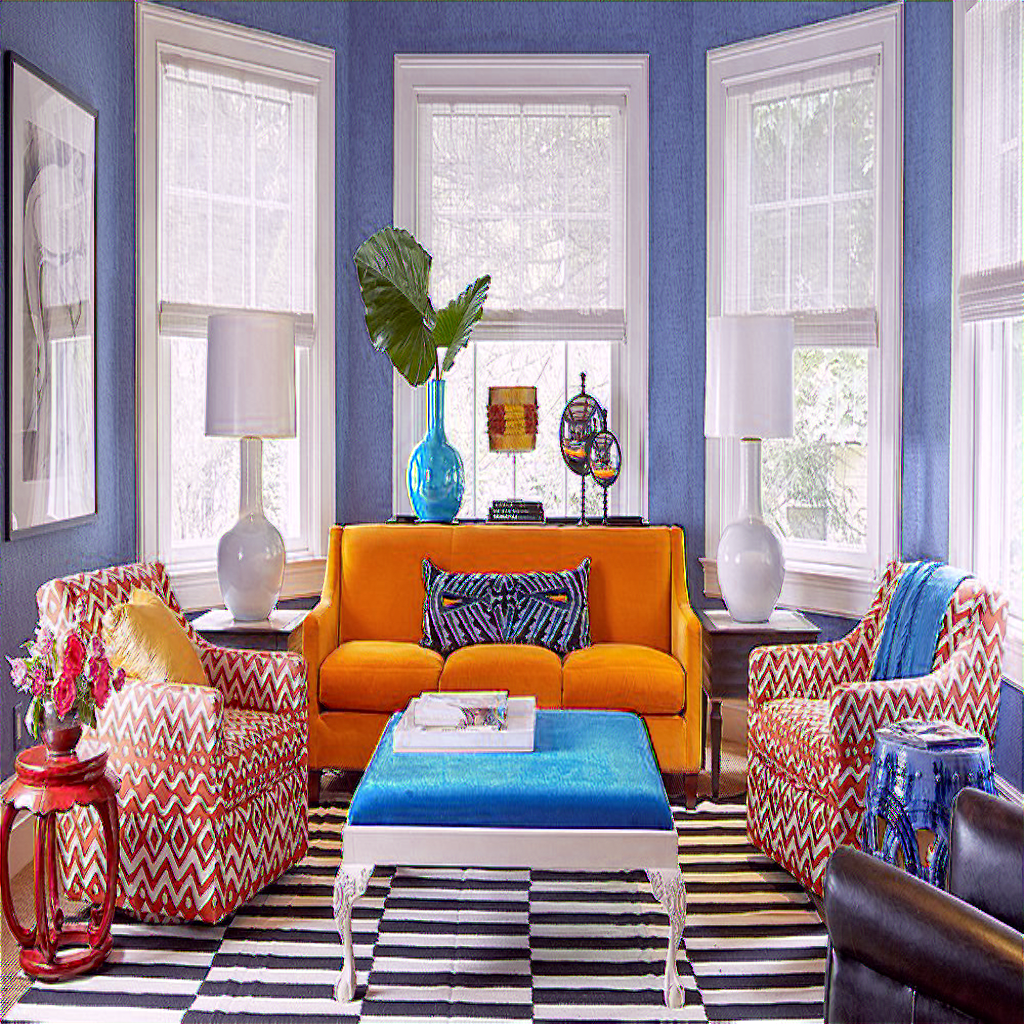
\includegraphics[width=\linewidth]{reconst_exper/dec_room_my_1_test.png} % our reconstruction num.5
		\caption{Ours arc1}
	\end{subfigure}
	\begin{subfigure}[b]{0.13\linewidth}
		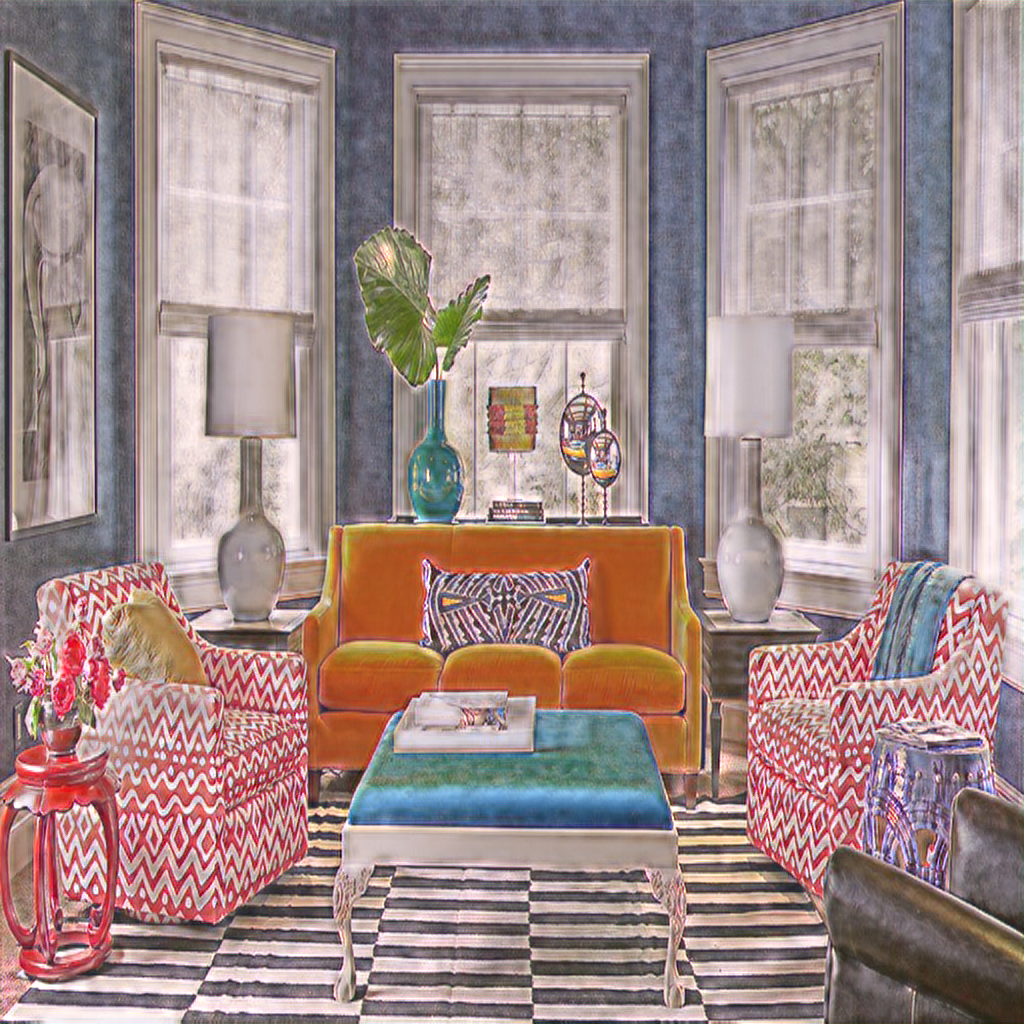
\includegraphics[width=\linewidth]{reconst_exper/dec_room_my_2_test.png} % our reconstruction num.5
		\caption{Ours arc2}
	\end{subfigure}
	\begin{subfigure}[b]{0.13\linewidth}
		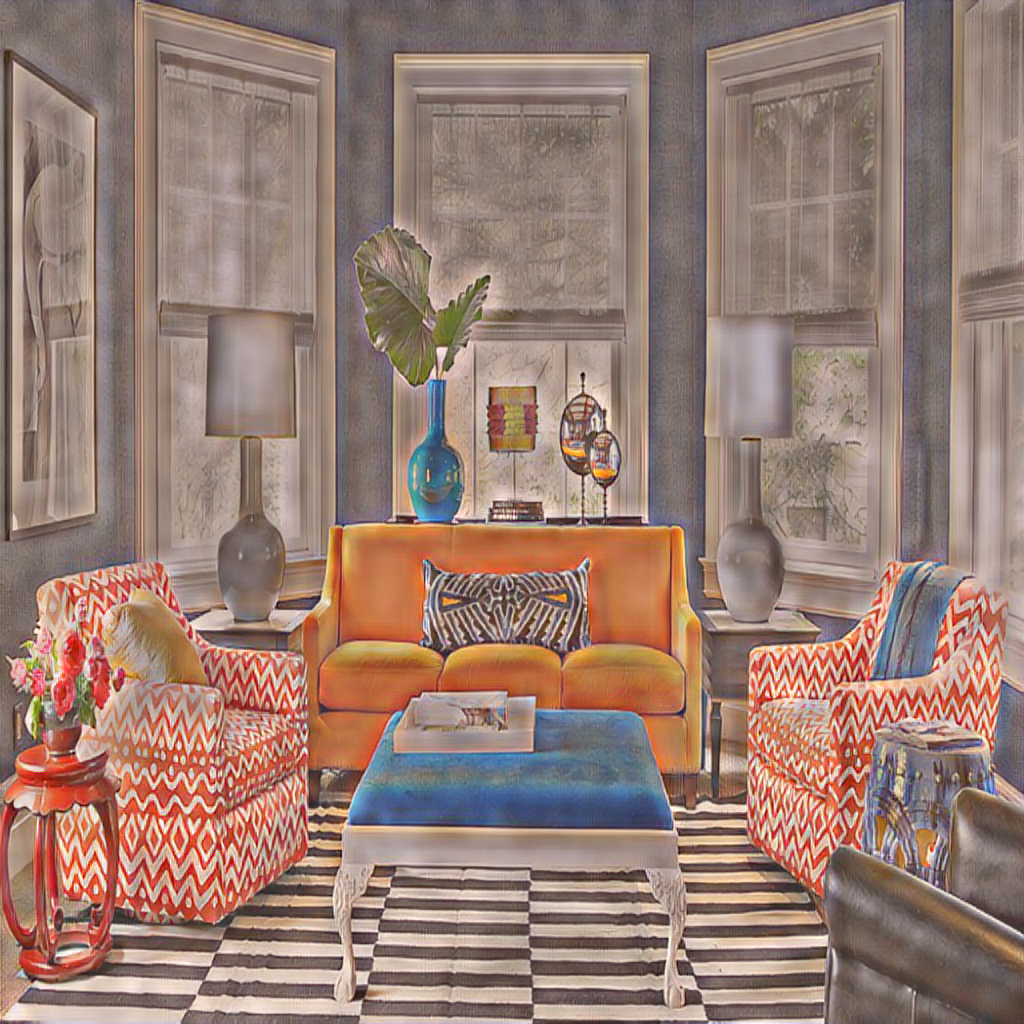
\includegraphics[width=\linewidth]{reconst_exper/dec_room_my_3_test.png} % our reconstruction num.5
		\caption{Ours arc3}
	\end{subfigure}
	\begin{subfigure}[b]{0.13\linewidth}
		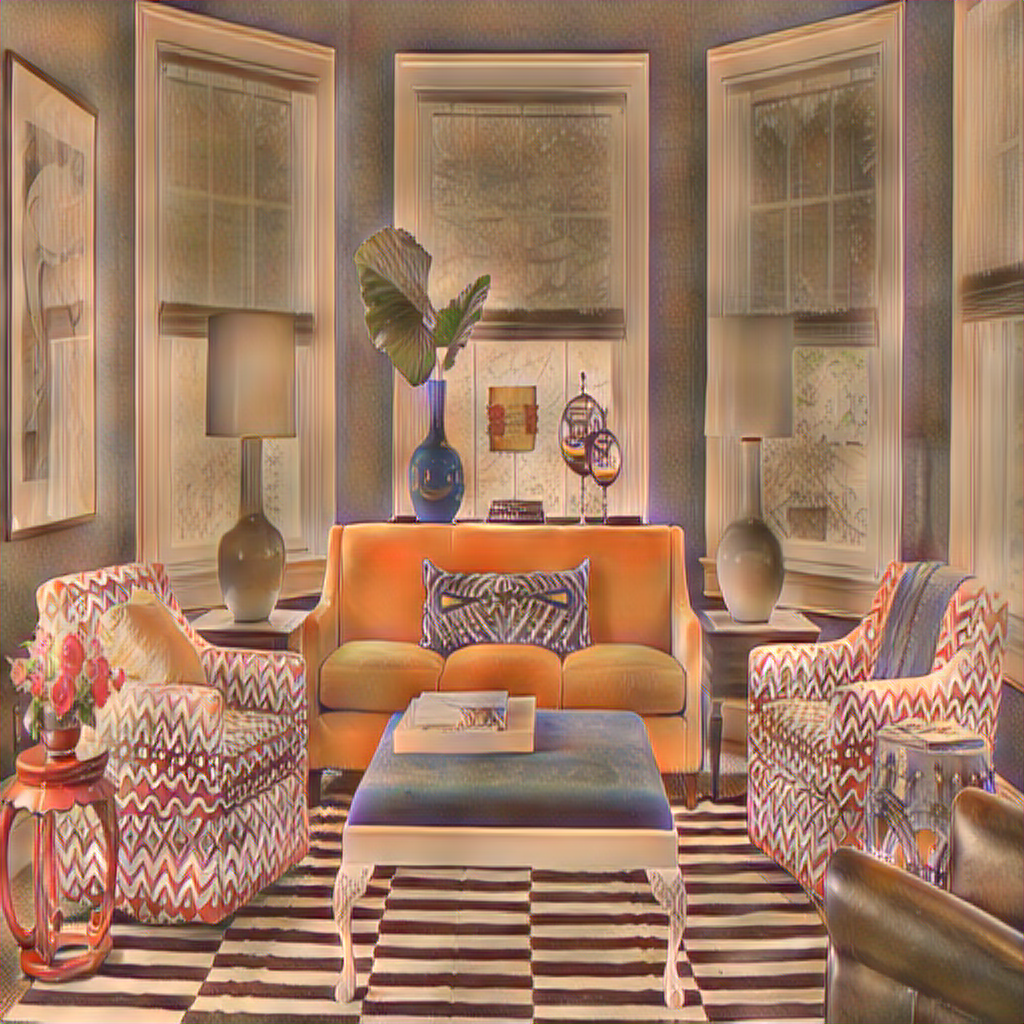
\includegraphics[width=\linewidth]{reconst_exper/dec_room_my_4_test.png} % our reconstruction num.5
		\caption{Ours arc4}
	\end{subfigure}
	\begin{subfigure}[b]{0.13\linewidth}
		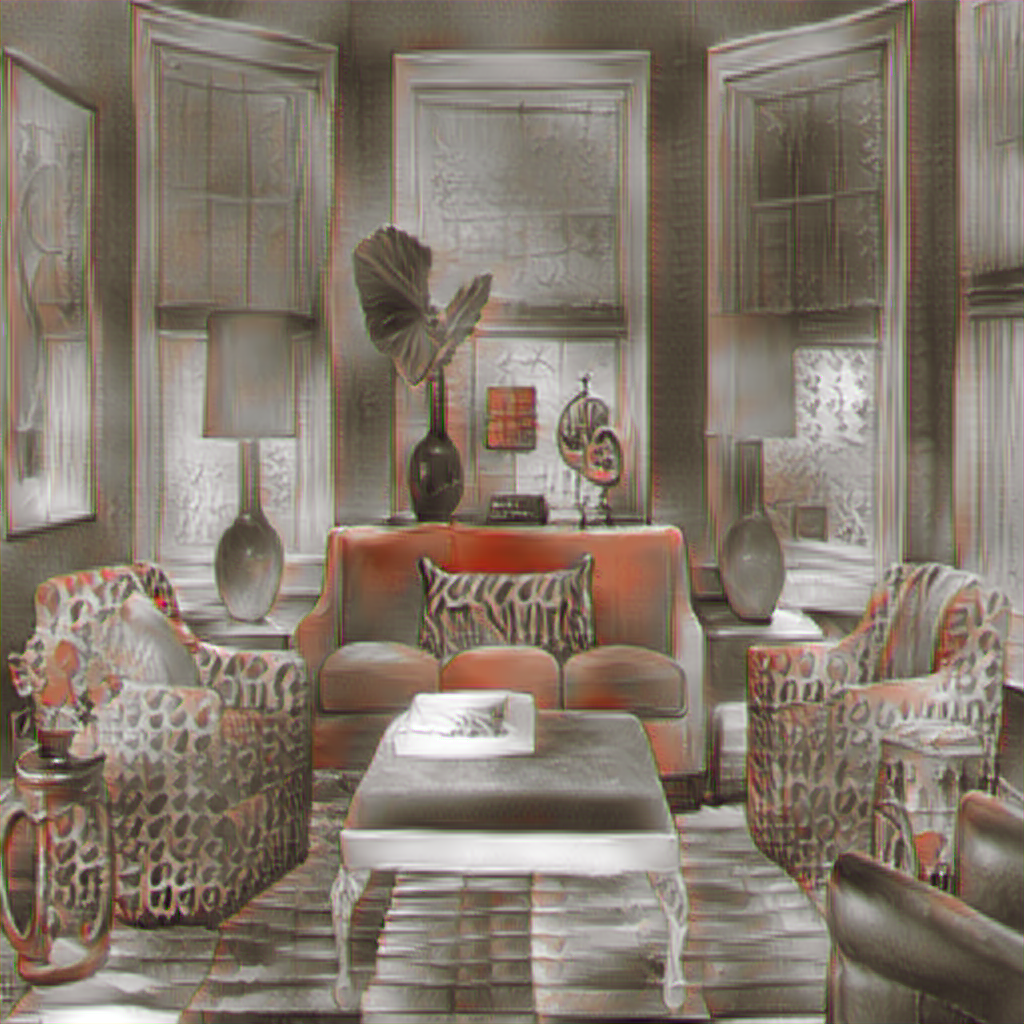
\includegraphics[width=\linewidth]{reconst_exper/dec_room_my_5_test.png} % our reconstruction num.5
		\caption{Ours arc5}
	\end{subfigure}
	\begin{subfigure}[b]{0.13\linewidth}
		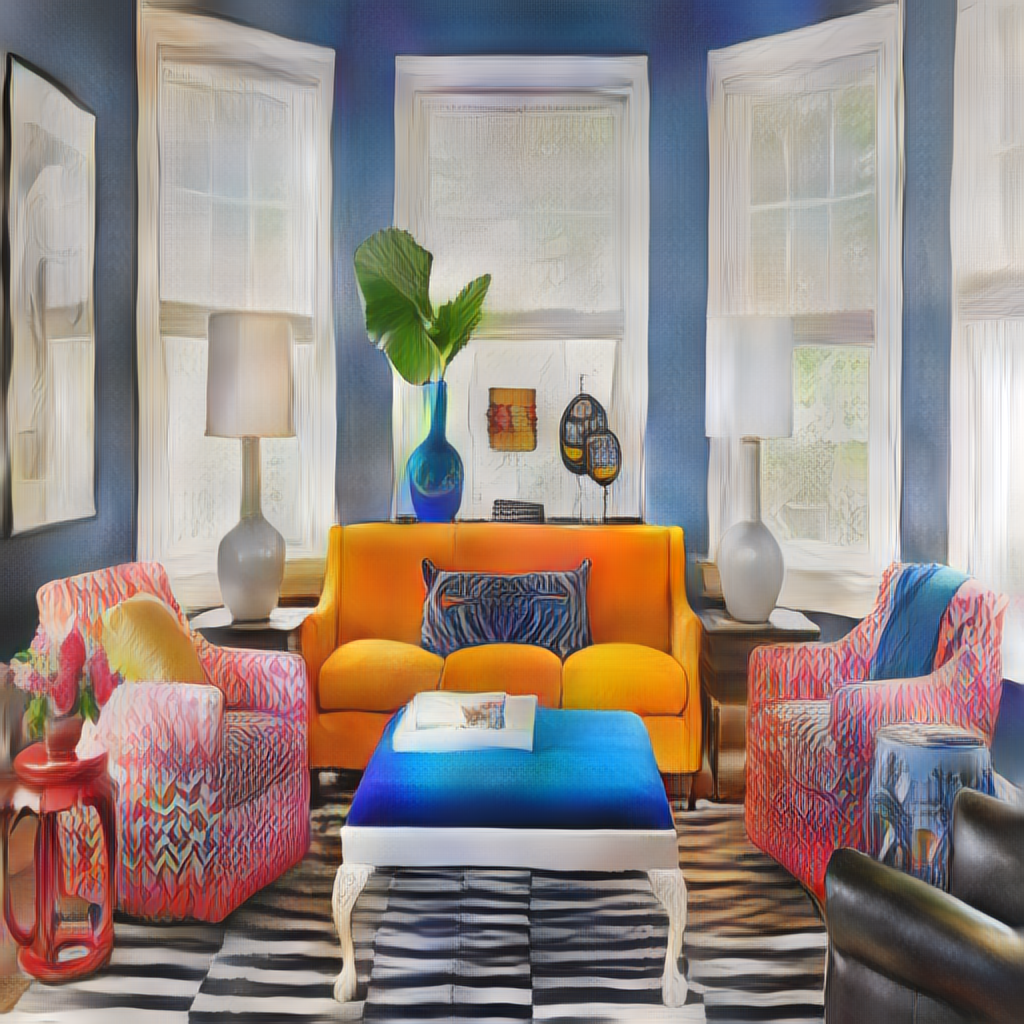
\includegraphics[width=\linewidth]{reconst_exper/dec_room_ref_5_test.png} % their reconstruction arc5 num.1
		\caption{Ref arc5}	
	\end{subfigure}
	\caption{Reconstructed images}
	\label{fig:reconstruction}
\end{figure}
Figure ~\ref{fig:reconstruction} shows reconstruction of original images (figure ~\ref{fig:reconstruction} (a)) using different architectures of encoder-decoder, i.e. figure ~\ref{fig:reconstruction} (b) uses architecture 1 which uses Encoder-1 and Decoder-Block-1, figure ~\ref{fig:reconstruction} (c) uses architecture 3 which uses Encoder-3 and Decoder-Block-3, etc. as depicted in \ref{subsec:Models}.

\subsubsection{TODO}
Our distortion-of-reconstruction loss table ~\ref{Tab:loss} shows by both pixel and feature loss, that the first architecture has the less loss since it is only uses 1 convolution layer. As we go deeper in architectures in a manner of convolutional layers, we see that the loss arises respectively. Hence we decided to balance the distortion in out continuous work, therefore we chose to work with a pipeline that has architecture 4, forsake architecture 5 to avoid major distortion such as smoothing and blurring artifacts.

As part of implementing UST \cite{bib11}, we separately train five reconstruction decoders for features
at the VGG-19 \verb|Relu_X_1| (X=1,2,...,5) layers. It is trained on the Microsoft COCO dataset \cite{bib10} and
the weight $\lambda$ to balance the two losses in (2) is set as 1.
The pixel reconstruction loss \cite{bib22} and feature loss \cite{bib22, bib17} are employed for reconstructing an input image, see equation ~\ref{eq:loss}
After training, the decoder is fixed (i.e., will not be fine-tuned) and used as a feature inverter.\newline
%%%%%%%%%%%%%%%%%%%%%%%%%%%%%%%%%%%%%%%%%%
%%% recunstruction comparison %%%
%%%%%%%%%%%%%%%%%%%%%%%%%%%%%%%%%%%%%%%%%%
Section \ref{subsec:Decoders} explains why we needed to train 5 different decoders. Without time and compute power limitations we could get much more powerful decoders which are not producing such as artifacts.
In addition, we measure quantitatively (see table ~\ref{Tab:loss}) our reconstruction distortion loss by two measures: pixel loss and feature loss as depicted in equation \ref{eq:loss} and elaborated in \cite{bib22, bib17}.\newline\\

%%%%%%%%%%%%%%%%%%%%%%%%%%%%%% Reconstrucion images %%%%%%%%%%%%%%%%%%%%%%%%%%%%%%%%%%

  
%%%%%%%%%%%%%%%%%%%%%%%%%%%%
%%%%%%%%%%%%%%%%%%%%%%%%%%%%
% style transfer images %
%%%%%%%%%%%%%%%%%%%%%%%%%%%%
%%%%%%%%%%%%%%%%%%%%%%%%%%%%
\subsection{Style Transfer Experimental Results}
\begin{figure}[H]
	% first line
	\centering
	\begin{subfigure}[b]{0.225\linewidth}
		
\includegraphics[width=\linewidth]{bridge_sq.jpg} % style img num.1
	\end{subfigure}
	\begin{subfigure}[b]{0.225\linewidth}
		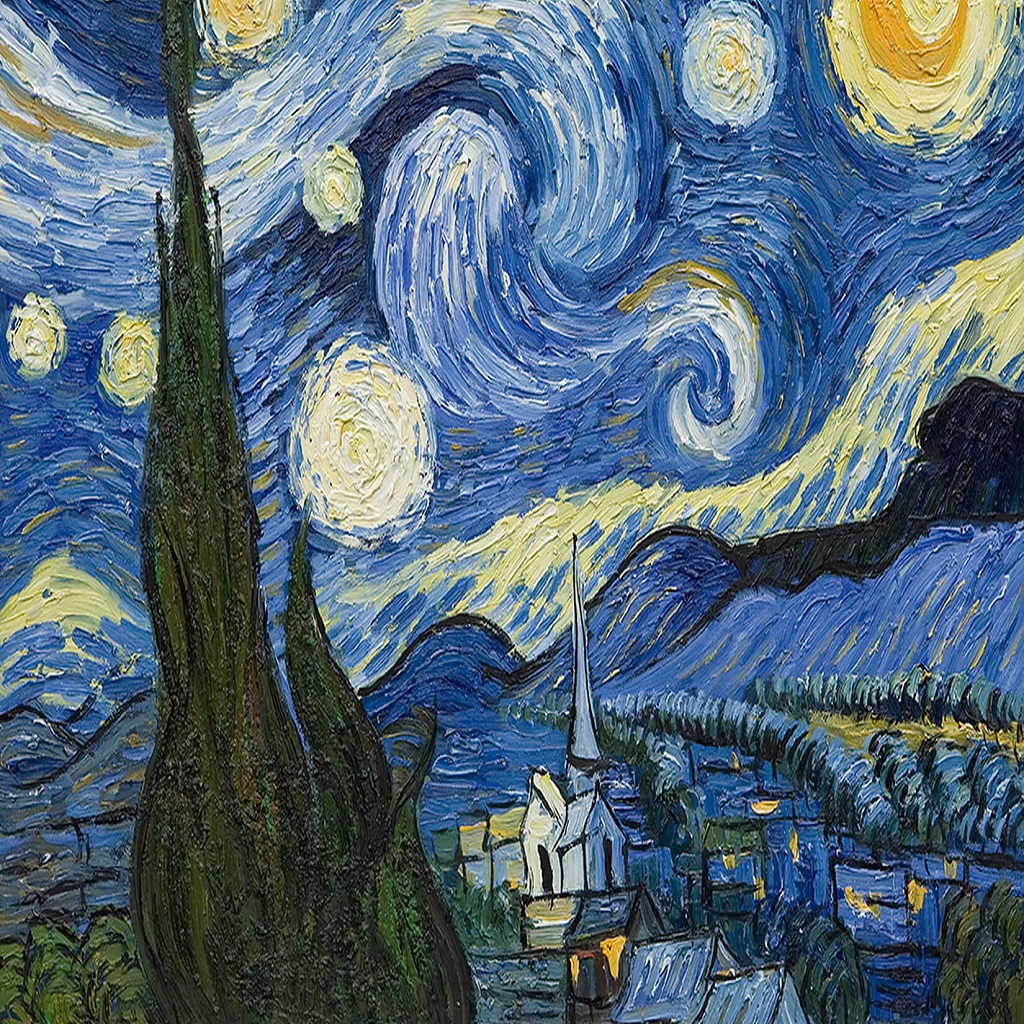
\includegraphics[width=\linewidth]{starry_sq.jpg} % content img num.1	
	\end{subfigure}
	\begin{subfigure}[b]{0.225\linewidth}
		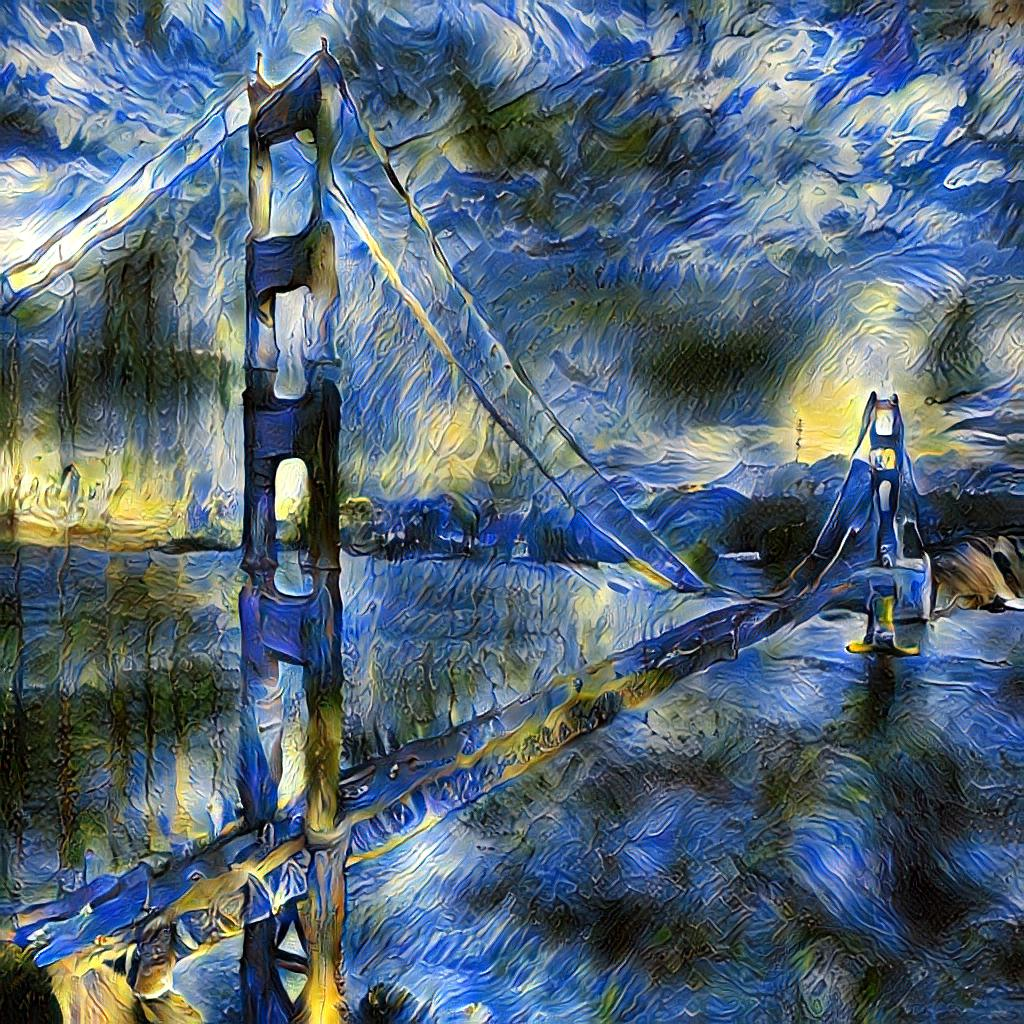
\includegraphics[width=\linewidth]{transfer_examples/transfer_bridge_starry_08_ref.jpg} % theirs reconstruction num.1	
	\end{subfigure}
	\begin{subfigure}[b]{0.225\linewidth}
		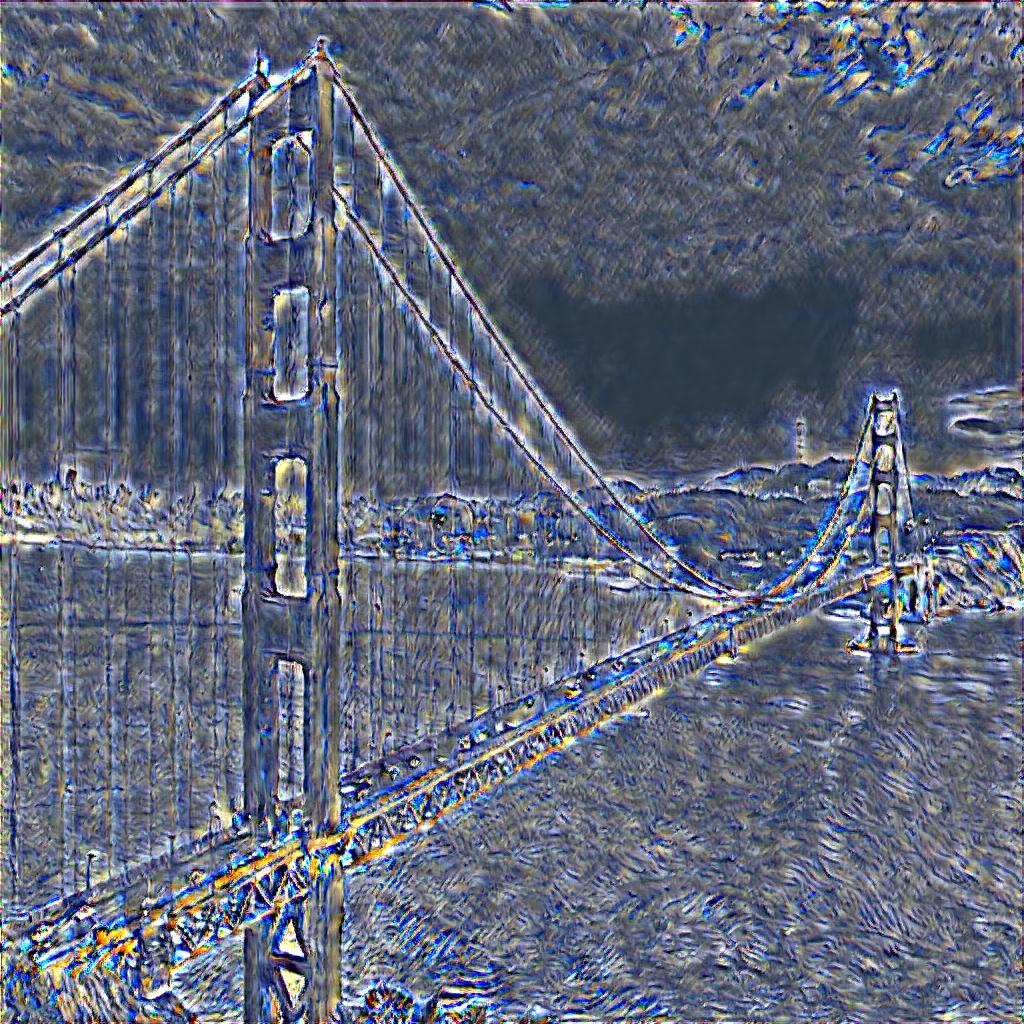
\includegraphics[width=\linewidth]{transfer_examples/transfer_bridge_starry_08_our.jpg} % ours reconstruction num.1	
	\end{subfigure}
	% second line
	\centering
	\begin{subfigure}[b]{0.225\linewidth}
		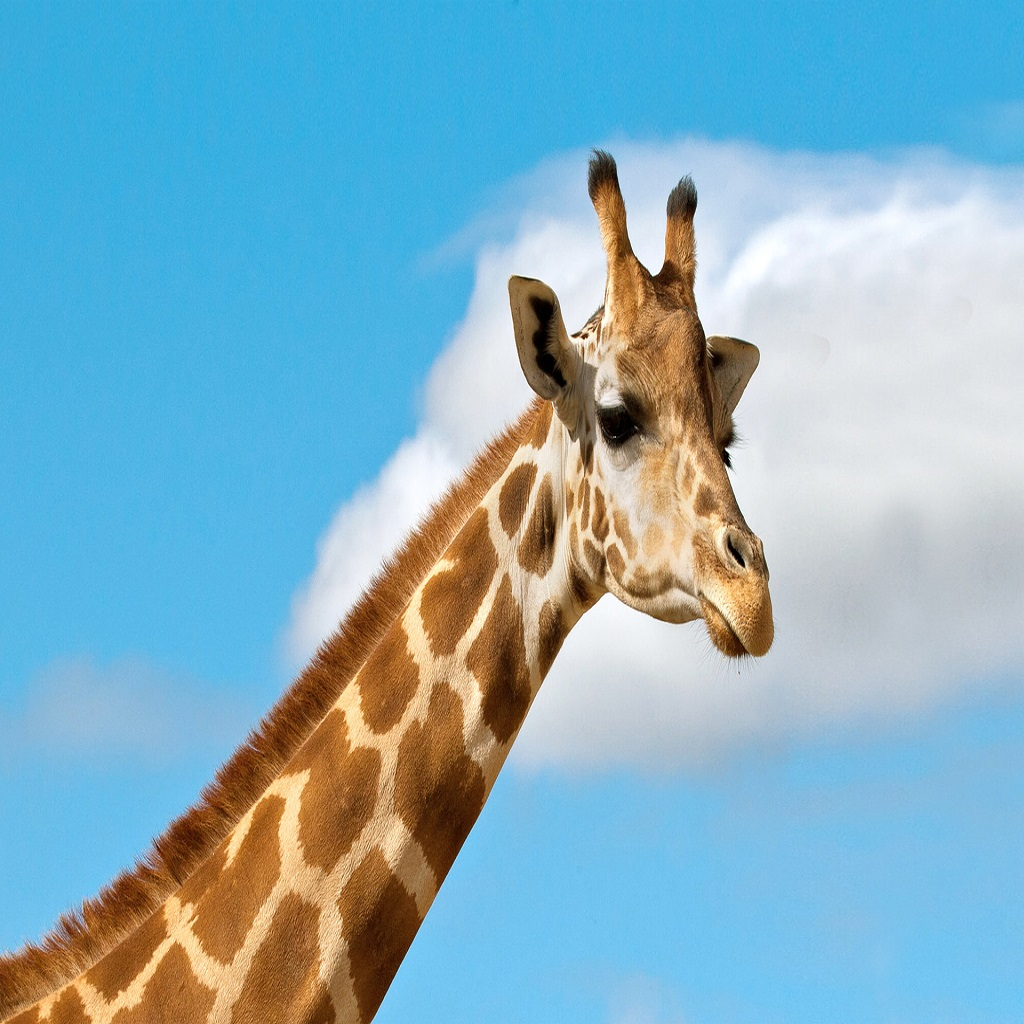
\includegraphics[width=\linewidth]{giraffe_sq.jpg} %style img num.2
	\end{subfigure}
	\begin{subfigure}[b]{0.225\linewidth}
		
\includegraphics[width=\linewidth]{st1_sq.jpg} % content img num.2
	\end{subfigure}
	\begin{subfigure}[b]{0.225\linewidth}
		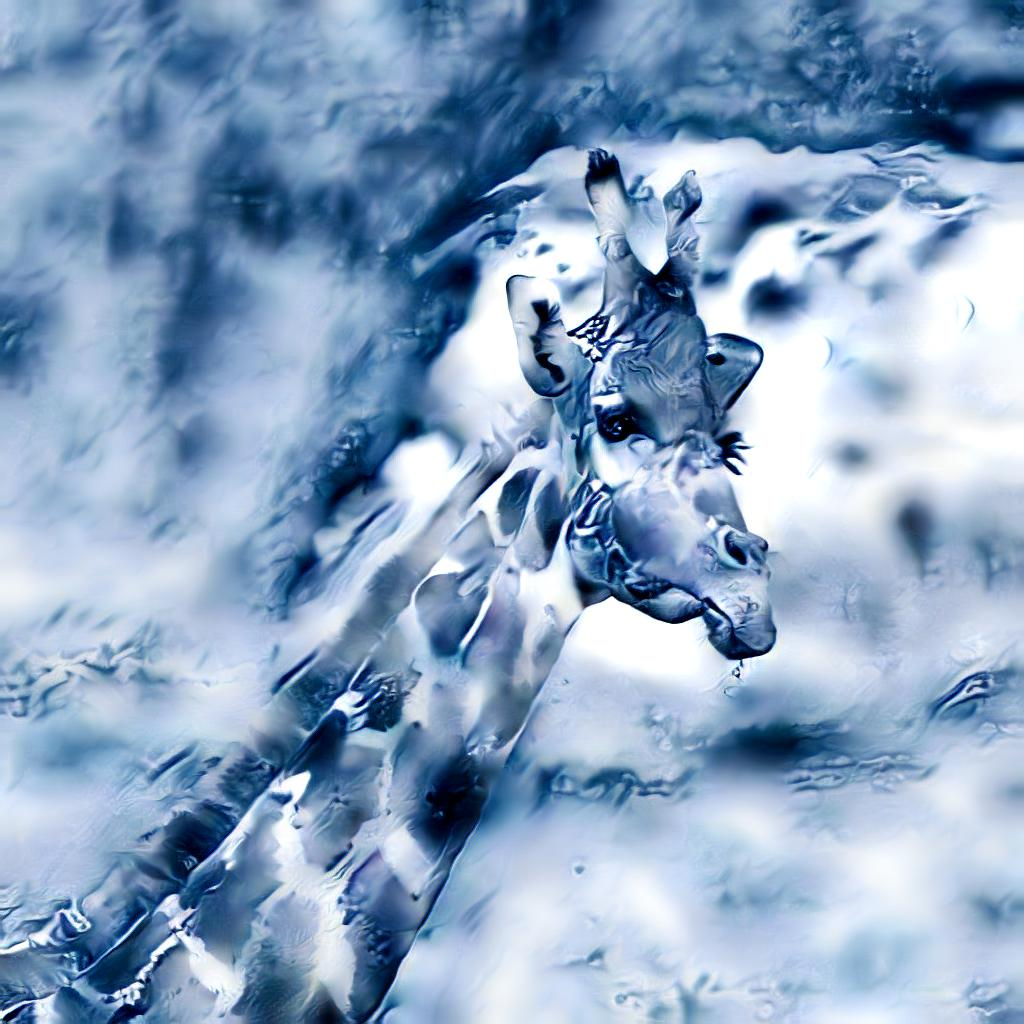
\includegraphics[width=\linewidth]{transfer_examples/transfer_giraffe_st1_08_ref.jpg} % theirs reconstruction num.2
	\end{subfigure}
	\begin{subfigure}[b]{0.225\linewidth}
		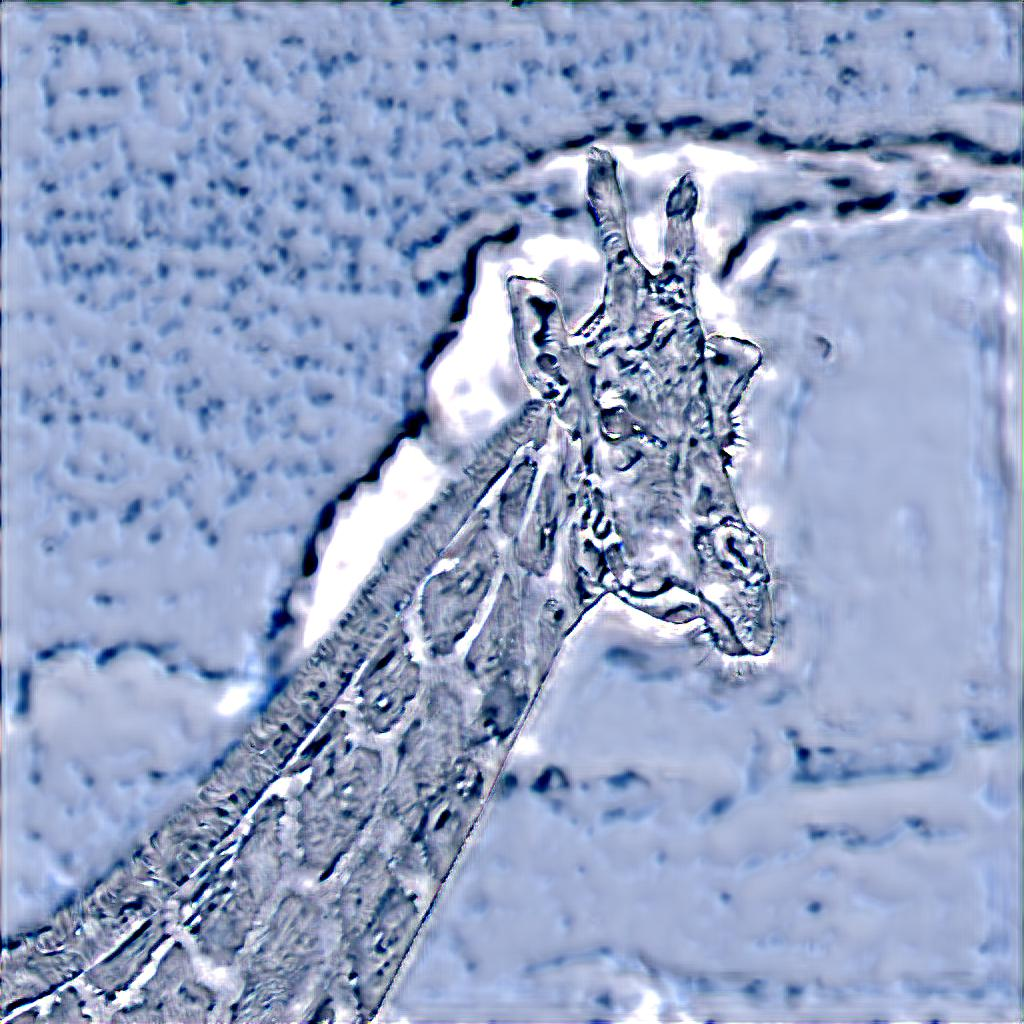
\includegraphics[width=\linewidth]{transfer_examples/transfer_giraffe_st1_08_our.jpg} % ours reconstruction num.2
	\end{subfigure}
	% third line
	\centering
	\begin{subfigure}[b]{0.225\linewidth}
		
\includegraphics[width=\linewidth]{in1_sq.jpg} %style img num.3
	\end{subfigure}
	\begin{subfigure}[b]{0.225\linewidth}
		
\includegraphics[width=\linewidth]{tiger_sq.jpg} % content img num.3
	\end{subfigure}
	\begin{subfigure}[b]{0.225\linewidth}
		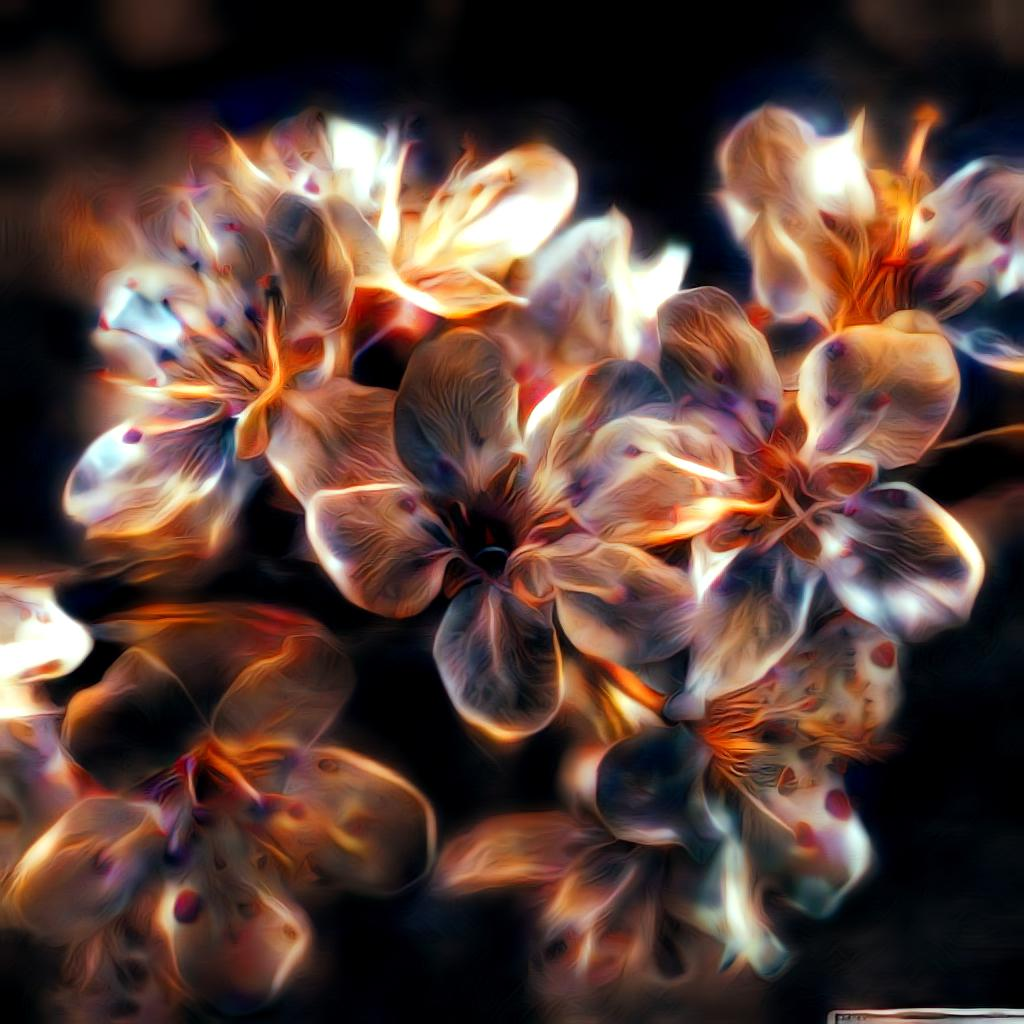
\includegraphics[width=\linewidth]{transfer_examples/transfer_in1_tiger_08_ref.jpg} % theirs reconstruction num.3
	\end{subfigure}
	\begin{subfigure}[b]{0.225\linewidth}
		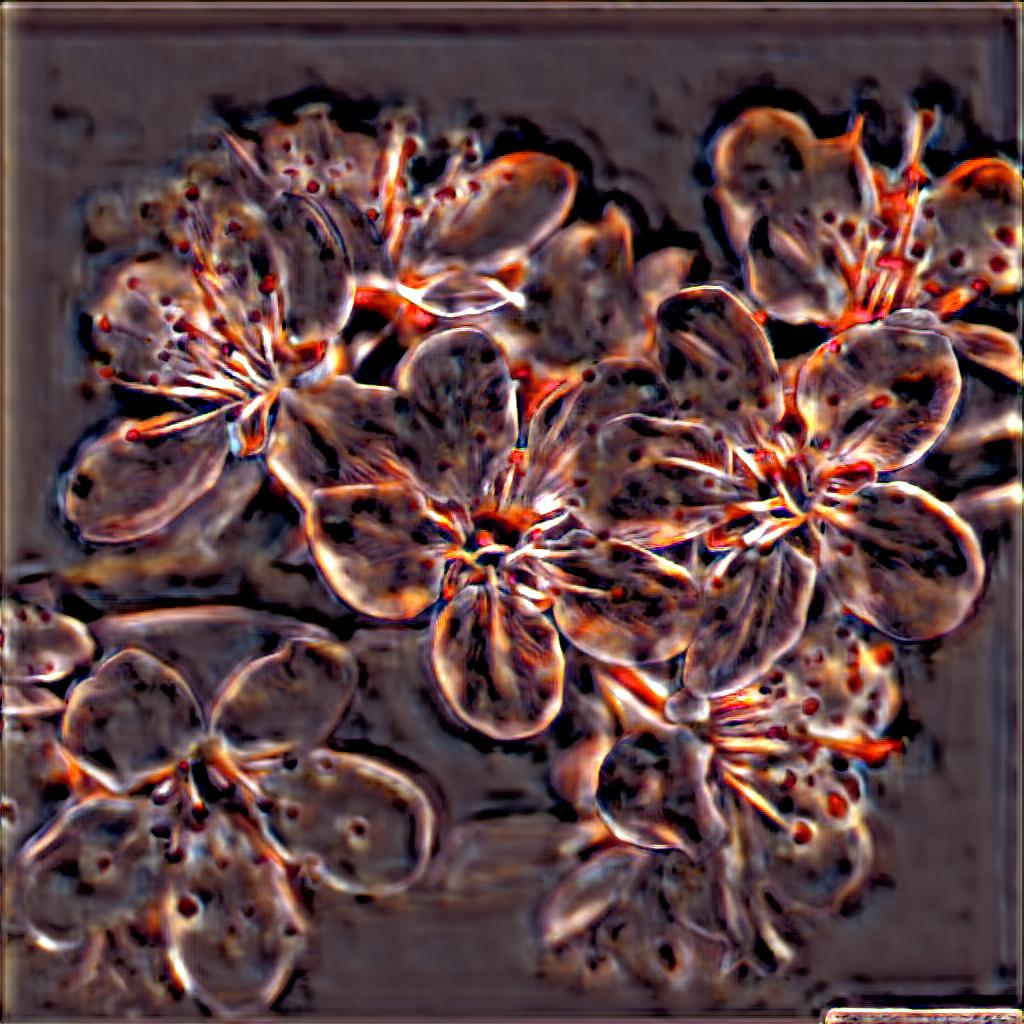
\includegraphics[width=\linewidth]{transfer_examples/transfer_in1_tiger_08_our.jpg} % ours reconstruction num.3
	\end{subfigure}
	% fourth line
	\centering
	\begin{subfigure}[b]{0.225\linewidth}
		\includegraphics[width=\linewidth]{nyc_sq.jpg} %style img num.4
	\end{subfigure}
	\begin{subfigure}[b]{0.225\linewidth}
		\includegraphics[width=\linewidth]{graffiti_sq.jpg} % content img num.4
	\end{subfigure}
	\begin{subfigure}[b]{0.225\linewidth}
		\includegraphics[width=\linewidth]{transfer_examples/transfer_nyc_graffiti_08_ref.jpg} % theirs reconstruction num.4
	\end{subfigure}
	\begin{subfigure}[b]{0.225\linewidth}
		\includegraphics[width=\linewidth]{transfer_examples/transfer_nyc_graffiti_08_our.jpg} % ours reconstruction num.4
	\end{subfigure}
	% fifth line
	\centering
	\begin{subfigure}[b]{0.225\linewidth}
		\includegraphics[width=\linewidth]{room_sq.jpg} %style img num.5
		\caption{Content}
	\end{subfigure}
	\begin{subfigure}[b]{0.225\linewidth}
		\includegraphics[width=\linewidth]{st2_sq.jpg} % content img num.5
		\caption{Style}
	\end{subfigure}
	\begin{subfigure}[b]{0.225\linewidth}
		\includegraphics[width=\linewidth]{transfer_examples/transfer_room_paint_08_ref.jpg} % theirs reconstruction num.5
		\caption{Reference Models}
	\end{subfigure}
	\begin{subfigure}[b]{0.225\linewidth}
		\includegraphics[width=\linewidth]{transfer_examples/transfer_room_paint_08_our.jpg} % ours reconstruction num.5
		\caption{Our Models}
	\end{subfigure}
	\caption{Results from different style transfer methods using style weight $\alpha=0.5$}
	\label{fig:style_transfer}
\end{figure}
%%%%%%%%%%%%%%%%%%%%%%%%%%%%
%%%%%%%%%%%%%%%%%%%%%%%%%%%%
% Boost %
%%%%%%%%%%%%%%%%%%%%%%%%%%%%
%%%%%%%%%%%%%%%%%%%%%%%%%%%%
\subsubsection{Stylization boosting}
\begin{figure}[H]
	% first line
	\centering
	\begin{subfigure}[b]{0.4\linewidth}
		\includegraphics[width=\linewidth]{car.jpg} %style img num.1
		\caption{Content}
	\end{subfigure}
	\begin{subfigure}[b]{0.4\linewidth}
		\includegraphics[width=\linewidth]{car.jpg} % content img num.1
		\caption{Style}
	\end{subfigure}
	%second line
	\begin{subfigure}[b]{0.4\linewidth}
		\includegraphics[width=\linewidth]{car.jpg} % regular UST num.1
		\caption{Regular UST}
	\end{subfigure}
	\begin{subfigure}[b]{0.4\linewidth}
		\includegraphics[width=\linewidth]{car.jpg} % UST+boost num.1
		\caption{Boost UST}
	\end{subfigure}
	\centering
	\begin{subfigure}[b]{0.4\linewidth}
		\includegraphics[width=\linewidth]{car.jpg} %style img num.1
		\caption{Content}
	\end{subfigure}
	\begin{subfigure}[b]{0.4\linewidth}
		\includegraphics[width=\linewidth]{car.jpg} % content img num.1
		\caption{Style}
	\end{subfigure}
	%second line
	\begin{subfigure}[b]{0.4\linewidth}
		\includegraphics[width=\linewidth]{car.jpg} % regular UST num.1
		\caption{Regular UST}
	\end{subfigure}
	\begin{subfigure}[b]{0.4\linewidth}
		\includegraphics[width=\linewidth]{car.jpg} % UST+boost num.1
		\caption{Boost UST}
	\end{subfigure}
	\caption{Boosting results comparing to original UST \cite{bib11}.}
	\label{fig:Boost}
\end{figure}
%%%%%%%%%%%%%%%%%%%%%%%% Merge  %%%%%%%%%%%%%%%%%%%%%%
\subsubsection{Two styles merging methods}
\begin{figure}[H]
	% first line
	\centering
	\begin{subfigure}[b]{0.13\linewidth}
		\includegraphics[width=\linewidth]{car.jpg} %style img num.1
	\end{subfigure}
	\begin{subfigure}[b]{0.13\linewidth}
		\includegraphics[width=\linewidth]{car.jpg} % style2 img num.1
	\end{subfigure}
	\begin{subfigure}[b]{0.13\linewidth}
		\includegraphics[width=\linewidth]{car.jpg} % content img num.1
	\end{subfigure}
	\begin{subfigure}[b]{0.13\linewidth}
		\includegraphics[width=\linewidth]{car.jpg} % orig merge num.1
	\end{subfigure}
	\begin{subfigure}[b]{0.13\linewidth}
		\includegraphics[width=\linewidth]{car.jpg} % merge1 num.1
	\end{subfigure}
	\begin{subfigure}[b]{0.13\linewidth}
		\includegraphics[width=\linewidth]{car.jpg} % merge2 num.1
	\end{subfigure}
	\begin{subfigure}[b]{0.13\linewidth}
		\includegraphics[width=\linewidth]{car.jpg} % merge3 num.1
	\end{subfigure}
	% second line
	\centering
	\begin{subfigure}[b]{0.13\linewidth}
		\includegraphics[width=\linewidth]{car.jpg} %style img num.2
	\end{subfigure}
	\begin{subfigure}[b]{0.13\linewidth}
		\includegraphics[width=\linewidth]{car.jpg} % style2 img num.2
	\end{subfigure}
	\begin{subfigure}[b]{0.13\linewidth}
		\includegraphics[width=\linewidth]{car.jpg} % content img num.2
	\end{subfigure}
	\begin{subfigure}[b]{0.13\linewidth}
		\includegraphics[width=\linewidth]{car.jpg} % orig merge num.2
	\end{subfigure}
	\begin{subfigure}[b]{0.13\linewidth}
		\includegraphics[width=\linewidth]{car.jpg} % merge1 num.2
	\end{subfigure}
	\begin{subfigure}[b]{0.13\linewidth}
		\includegraphics[width=\linewidth]{car.jpg} % merge2 num.2
	\end{subfigure}
	\begin{subfigure}[b]{0.13\linewidth}
		\includegraphics[width=\linewidth]{car.jpg} % merge3 num.2
	\end{subfigure}
	% third line
	\centering
	\begin{subfigure}[b]{0.13\linewidth}
		\includegraphics[width=\linewidth]{car.jpg} %style img num.3
		\caption{$1_{st}$ \\ Style}
	\end{subfigure}
	\begin{subfigure}[b]{0.13\linewidth}
		\includegraphics[width=\linewidth]{car.jpg} %style2 img num.3
		\caption{$2_{nd}$ \\ Style}
	\end{subfigure}
	\begin{subfigure}[b]{0.13\linewidth}
		\includegraphics[width=\linewidth]{car.jpg} % content img num.3
		\caption{Content \\ image}
	\end{subfigure}
	\begin{subfigure}[b]{0.13\linewidth}
		\includegraphics[width=\linewidth]{car.jpg} % orig merge num.3
		\caption{Li et al. \cite{bib11}}
	\end{subfigure}
	\begin{subfigure}[b]{0.13\linewidth}
		\includegraphics[width=\linewidth]{car.jpg} % merge1 num.3
		\caption{$1_{st}$ method}
	\end{subfigure}
	\begin{subfigure}[b]{0.13\linewidth}
		\includegraphics[width=\linewidth]{car.jpg} % merge2 num.3
		\caption{$2_{nd}$ method}
	\end{subfigure}
	\begin{subfigure}[b]{0.13\linewidth}
		\includegraphics[width=\linewidth]{car.jpg} % merge3 num.3
		\caption{$3_{rd}$ method}
	\end{subfigure}
		\caption{Results using different stylization methods. (d) is the original merge method as in \cite{bib11}, (e) is Level Merge, (f) is Channel Merge and (g) is Interpolate-Style Merge.}
		\label{fig:Merge}
\end{figure}
%%%%%%%%%%%%%%%%%%%%%%%%%%%%
add more text here
%%%%%%%%%%%%%%%%%%%%%%%% Texture synthesis  %%%%%%%%%%%%%%%%%%%%%%
\subsubsection{Texture synthesis}
We demonstrate the effectiveness of our method for universal style transfer by showing its application to universal texture synthesis. In figure ~\ref{fig:texture} we visualize the whitened features and
synthesized textures via simple feature coloring.
One option to produce texture image is simply setting the content image as a random noise image (e.g., Gaussian noise). Another option to get synthesized texture in our stylization framework is to directly initialize the content features to be white noise as proposed by Li et al. \cite{bib11}. Both approaches achieve similar results.
The evaluation criterion for the quality of the synthesized texture is usually human inspection and textures are successfully synthesized if a human observer cannot tell the original texture from a synthesized one.
\begin{figure}[H]
	% first line
	\centering
	\begin{subfigure}[b]{0.4\linewidth}
		\includegraphics[width=\linewidth]{car.jpg} %texture img num.1
	\end{subfigure}
	\begin{subfigure}[b]{0.4\linewidth}
		\includegraphics[width=\linewidth]{car.jpg} % content img num.1
	\end{subfigure}
	% second line
	\centering
	\begin{subfigure}[b]{0.4\linewidth}
		\includegraphics[width=\linewidth]{car.jpg} %content img num.3
		\caption{Style}
	\end{subfigure}
	\begin{subfigure}[b]{0.4\linewidth}
		\includegraphics[width=\linewidth]{car.jpg} % stylization img num.3
		\caption{Our UST}
	\end{subfigure}
	\caption{Synthesized results using our UST implementation.}
	\label{fig:texture}
\end{figure}
	
	\section{Conclusions}
	\label{conclusions_lbl}
	\input{conclusions}
		
	%\section{References}
	\label{references_lbl}
	\begin{thebibliography}{9}
\bibitem{bib1}
A. Efros and T. K. Leung.  Texture synthesis by non-parametric sampling. In Computer Vision, 1999. The Proceedings of the Seventh IEEE International Conference on,volume 2, pages 1033–1038. IEEE, 1999.

\bibitem{bib2}
L. Wei and M. Levoy.  Fast texture synthesis using tree-structured vector quantization. In Proceedings of the 27th annual conference on Computer graphics and interactive techniques, pages 479–488. ACM Press/Addison-Wesley Publishing Co., 2000.

\bibitem{bib3}
A. A. Efros and W. T. Freeman.  Image quilting for texture synthesis and transfer. In Proceedings of the 28th annual conference on Computer graphics and interactive techniques, pages 341–346. ACM, 2001.

\bibitem{bib4}
V. Kwatra, A. Schodl, I. Essa, G. Turk, and A. Bobick. Graph cut textures: image and video synthesis using graph cuts. In ACM Transactions on Graphics (ToG), volume 22,pages 277–286. ACM, 2003.

\bibitem{bib5}
H. Lee, S. Seo, S. Ryoo, and K. Yoon. Directional Texture Transfer. In Proceedings of the 8th International Symposium on Non-Photo realistic Animation and Rendering, NPAR ’10,pages 43–48, New York, NY, USA, 2010. ACM.

\bibitem{bib6}
A. Krizhevsky, I. Sutskever, and G. E. Hinton.  Image net classification with deep convolutional neural networks. In Advances in neural information processing systems, pages1097–1105, 2012.

\bibitem{bib7}
J. Donahue, Y. Jia, O. Vinyals, J. Hoffman, N. Zhang,E. Tzeng, and T. Darrell.   DeCAF: A Deep Convolutional Activation Feature for Generic Visual Recognition.arXiv:1310.1531 [cs], Oct. 2013. arXiv: 1310.1531

\bibitem{bib8}
M. Cimpoi, S. Maji, and A. Vedaldi. Deep filter banks for texture recognition and segmentation. In Proceedings of the IEEE Conference on Computer Vision and Pattern Recognition, pages 3828–3836, 2015.

\bibitem{bib9}
S. Karayev, M. Trentacoste, H. Han, A. Agarwala, T. Darrell,A. Hertzmann, and H. Winnemoeller.  Recognizing imagestyle.arXiv preprint arXiv:1311.3715, 2013.

\bibitem{bib10}
Lin, T.Y., Maire, M., Belongie, S., Hays, J., Perona, P., Ramanan, D., Dollar, P.,Zitnick, C.L.:  Microsoft COCO: Common objects in context.  In: ECCV, 2014. 

\bibitem{bib11}
[11] Li, Y., Fang, C., Yang, J., Wang, Z., Lu, X., Yang, M.H.:  Universal style transfer via feature transforms.  In: NIPS, 2017. 

\bibitem{bib12}
[12] Reinhard, E., Ashikhmin, M., Gooch, B., Shirley, P.: Color transfer between images.IEEE Computer graphics and applications21(5) (2001) 34–41.

\bibitem{bib13}
[13] Freedman, D., Kisilev, P.:  Object-to-object color transfer: Optimal flows and smsp transformations.  In: CVPR, 2010. 

\bibitem{bib14}
[14] Shih,  Y.,  Paris,  S.,  Durand,  F.,  Freeman,  W.T.:   Data-driven  hallucination  of different times of day from a single outdoor photo.  In: SIGGRAPH, 2013.  

\bibitem{bib15}
[15] Li,  C.,  Wand,  M.:   Combining  markov  random  fields  and  convolutional  neural networks for image synthesis.  In: CVPR, 2016. 

\bibitem{bib16}
[16] Ulyanov, D., Lebedev, V., Vedaldi, A., Lempitsky, V.:  Texture networks: Feed-forward synthesis of textures and stylized images.  In: ICML, 2016.

\bibitem{bib17}
[17] Johnson, J., Alahi, A., Fei-Fei, L.:  Perceptual losses for real-time style transfer and super-resolution.  In: ECCV, 2016.

\bibitem{bib18}
Nikulin,  Y.,  Novak,  R.:  Exploring  the  neural  algorithm  of  artistic  style.  CoRRabs/1602.07188, 2016.

\bibitem{bib19}
X. Huang and S. Belongie. Arbitrary style transfer in real-time with adaptive instance normalization. In
ICCV, 2017.

\bibitem{bib20}
Simonyan, K., Zisserman, A.:  Very deep convolutional networks for large-scaleimage recognition.  In: ICLR, 2015.

\bibitem{bib21}
Deng, J., Dong, W., Socher, R., Li, L.-J., Li, K., and Fei-Fei, L.  Imagenet:  A large-scale hierarchical imagedatabase.  InProc. CVPR, 2009

\bibitem{bib22}
A. Dosovitskiy and T. Brox. Generating images with perceptual similarity metrics based on deep networks.
In NIPS, 2016.

\end{thebibliography}
\end{document}
